% !TeX encoding = UTF-8
% !TeX spellcheck = ru_RU
\documentclass[14pt,a4paper]{extarticle}

\usepackage{iftex}
\ifPDFTeX
  \usepackage[T2A]{fontenc}
  \usepackage[utf8]{inputenc}
  \usepackage[russian]{babel}
\else
  \usepackage{fontspec}
  \usepackage[russian]{babel}
  \IfFontExistsTF{Times New Roman}{\setmainfont{Times New Roman}}{\setmainfont{CMU Serif}}
  \IfFontExistsTF{Courier New}{\setmonofont{Courier New}}{\setmonofont{CMU Typewriter Text}}
\fi
\ifPDFTeX
  \usepackage{tempora}
  \usepackage{courier}
\fi

\usepackage[a4paper,left=30mm,right=10mm,top=20mm,bottom=20mm]{geometry}
\usepackage{setspace}
\usepackage{amsmath,amssymb}
\usepackage{graphicx}
\usepackage{tikz}
\usetikzlibrary{arrows.meta,positioning,shapes.geometric}
\usepackage{caption}
\usepackage{float}
\usepackage{array}
\usepackage{booktabs}
\usepackage{longtable}
\usepackage{tabularx}
\usepackage{multirow}
\usepackage{listings}
\usepackage{xcolor}
\usepackage{url}
\usepackage{hyperref}
\usepackage{kprj}

\VKRTitleOnly
\Ministry{Министерство науки и высшего образования\\Российской Федерации}
\BMSTU{Федеральное государственное автономное\\
образовательное учреждение высшего образования\\
\al{}Московский государственный технический университет\\
имени Н.\,Э.~Баумана (национальный\\
исследовательский университет)\ar{}\\
(МГТУ им. Н.Э.~Баумана)}
\title{Эвристические и ML-подходы к\\решению задачи 3D Bin Packing}
\author{И.В.~Иртюга}
\authorfull{Иртюга Илья Владимирович}
\group{ФН12-81Б}
\faculty{Фундаментальные науки}
\facultyshort{ФН}
\chair{Математическое моделирование}
\chairshort{ФН12}
\chief{Д.А.~Фетисов}
\inspector{\hspace{-1.5pt}М.А.~Велищанский}
\workyear{2026}

\onehalfspacing
\setcounter{secnumdepth}{3}
\setcontentsname{СОДЕРЖАНИЕ}
\setrefsname{СПИСОК ИСПОЛЬЗОВАННЫХ ИСТОЧНИКОВ}

\hypersetup{
  unicode=true,
  colorlinks=true,
  linkcolor=black,
  citecolor=black,
  urlcolor=black,
  pdfauthor={Иртюга Илья Владимирович},
  pdftitle={Эвристические и ML-подходы к решению задачи 3D Bin Packing}
}
\pdfstringdefDisableCommands{%
  \let\centering\empty
}

\captionsetup[figure]{labelsep=period,justification=centering}
\captionsetup[table]{labelsep=endash,justification=raggedright,singlelinecheck=false}
\makeatletter
\long\def\@makecaption#1#2{%
  \def\@tempa{#2}\def\@tempb{\ignorespaces}%
  \ifx\@tempa\@tempb
    \def\@tempb{{\captionnofont{#1}}}%
  \else
    \def\@tempc{table}%
    \ifx\@captype\@tempc
      \def\@tempb{{\captionnofont{#1~--}\space}}%
    \else
      \def\@tempb{{\captionnofont{#1.}\space}}%
    \fi
  \fi
  \sbox\@tempboxa{\captionfont\@tempb#2}%
  \ifdim \wd\@tempboxa >\hsize
    \def\@tempc{table}%
    \ifx\@captype\@tempc
      {\raggedright\captionfont\@tempb#2\par}%
    \else
      {\centering\captionfont\@tempb#2\par}%
    \fi
  \else
    \global \@minipagefalse
    \hb@xt@\hsize{\hfil\box\@tempboxa\hfil}%
  \fi}
\makeatother
\renewcommand{\arraystretch}{1.15}
\graphicspath{{images/}}
\sloppy

\lstset{
  basicstyle=\ttfamily\small,
  breaklines=true,
  columns=fullflexible,
  frame=single,
  keepspaces=true
}

\newcommand{\structsection}[1]{%
  \clearpage
  \section*{\MakeUppercase{#1}}%
  \addcontentsline{toc}{section}{\MakeUppercase{#1}}%
}
\newcommand{\code}[1]{\texttt{#1}}

\begin{document}

\begin{spacing}{1.0}
\maketitle
\end{spacing}

\structsection{Реферат}

Расчетно-пояснительная записка содержит 35 с., 8 рис., 9 табл., 11 источников, 2 приложения.

\textbf{Ключевые слова:} 3D BIN PACKING, ПАЛЛЕТИЗАЦИЯ, SMART 3D PACKING, ЭВРИСТИЧЕСКИЕ АЛГОРИТМЫ, LARGE NEIGHBORHOOD SEARCH, ГЕНЕТИЧЕСКИЙ АЛГОРИТМ, GAN, MAXRECTS, ЖАДНЫЙ АЛГОРИТМ, ВАЛИДАЦИЯ УКЛАДКИ.

Объектом исследования является программная система построения трехмерной укладки коробов на паллету. Предметом исследования являются эвристические, метаэвристические и ML-ориентированные методы решения задачи 3D Bin Packing в постановке Smart 3D Packing.

Цель выпускной квалификационной работы состоит в исследовании и сравнении реализованных подходов к решению задачи 3D Bin Packing с учетом прикладных ограничений складской логистики: габаритов паллеты, грузоподъемности, допустимых ориентаций, опоры, хрупкости товаров и времени расчета.

В работе рассмотрены постановка задачи, структура входных и выходных данных, метрика качества, генерация синтетических наборов данных, архитектура проекта и реализованные решатели. Подробно описаны жадный алгоритм на extreme points, послойный алгоритм на основе MaxRects, метаэвристика Large Neighborhood Search, гибридный метод GAN+GA, точный и ограниченный перебор для малых задач, а также многопаллетное расширение. Экспериментальная часть основана на сохраненных результатах проекта и едином валидаторе, что обеспечивает сопоставимость методов.

По результатам анализа установлено, что в single-pallet постановке на общих наборах данных наилучший средний итоговый score показывает LNS: 0.7111 на наборе из 100 задач, 0.7434 на наборе из 200 задач и 0.7298 на контрольном наборе. Преимущество LNS объясняется лучшим балансом между утилизацией объема, полнотой размещения, соблюдением ограничений хрупкости и временем выполнения.

\clearpage
\tableofcontents
\structsection{Введение}

Задача упаковки объектов в ограниченный контейнер является одной из классических задач комбинаторной оптимизации. В трехмерном варианте требуется разместить набор прямоугольных параллелепипедов внутри контейнера или на паллете так, чтобы объекты не пересекались и не выходили за заданные границы. В прикладной логистике такая задача возникает при сборке заказов, паллетизации товаров, загрузке транспорта и планировании складских операций.

В крупном ритейле качество паллетизации напрямую влияет на стоимость перевозки и устойчивость товарного потока. Недостаточно плотная укладка приводит к перевозке незаполненного объема, а неучет веса, хрупкости и устойчивости увеличивает риск повреждения товаров. Поэтому практическая постановка 3D Bin Packing существенно шире чисто геометрической задачи: необходимо одновременно учитывать размеры, массу, допустимые ориентации, опору снизу, возможность штабелирования и время расчета.

Тема настоящей выпускной квалификационной работы связана с проектом Smart 3D Packing. Условие проекта формулирует задачу построения алгоритмического модуля 3D Pallet Packing Optimizer, который по описанию паллеты и списка коробов возвращает план размещения с координатами и ориентациями каждого короба. Согласно условию, решение проходит двухэтапную проверку: сначала контролируются жесткие ограничения физической корректности, затем вычисляется взвешенная метрика качества.

Актуальность работы обусловлена тем, что задача 3D Bin Packing относится к NP-трудным задачам~\cite{martello2000}, а практически значимые экземпляры содержат десятки и сотни объектов. Полный перебор быстро становится неприменимым, поэтому в реальных системах используются эвристики, локальный поиск, метаэвристики и гибридные методы~\cite{faroe2003,pisinger2010}. В исследуемом проекте реализовано несколько таких подходов, что позволяет сравнить их в едином экспериментальном контуре.

\textbf{Цель работы} -- исследовать эвристические и ML-подходы к решению задачи 3D Bin Packing в проекте Smart 3D Packing и определить, какие методы обеспечивают лучший баланс качества укладки и времени расчета.

\textbf{Для достижения цели решаются следующие задачи:}
\begin{enumerate}
  \item изучить условие задачи Smart 3D Packing, требования к входным и выходным данным и правила валидации;
  \item формализовать ограничения и метрику качества упаковки;
  \item проанализировать структуру репозитория и восстановить pipeline решения;
  \item описать генерацию синтетических датасетов и состав используемых наборов данных;
  \item рассмотреть реализованные алгоритмы: greedy, MaxRects, LNS, GAN+GA, brute force и многопаллетное расширение;
  \item провести сравнительный анализ сохраненных экспериментальных результатов;
  \item сформулировать ограничения текущей реализации и направления дальнейшего развития.
\end{enumerate}

\textbf{Объект исследования} -- алгоритмическая система трехмерной укладки коробов на паллету.

\textbf{Предмет исследования} -- эвристические, метаэвристические и ML-ориентированные методы построения допустимой и качественной укладки в задаче 3D Bin Packing.

\textbf{Практическая значимость} работы заключается в том, что исследуемая система объединяет генератор данных, набор решателей, валидатор, средства визуализации и сохраненные benchmark-результаты. Такая структура может быть использована как основа для дальнейших исследований алгоритмов паллетизации и для прототипирования прикладного логистического модуля.

Работа состоит из введения, четырех разделов основной части, заключения, списка использованных источников и приложений. В первом разделе рассматриваются предметная область и постановка задачи. Во втором разделе приведен обзор методов решения 3D Bin Packing. В третьем разделе описана архитектура проекта Smart 3D Packing и реализация решателей. В четвертом разделе представлены датасеты, эксперименты, метрики и интерпретация результатов.

\clearpage
\section[\MakeUppercase{Анализ предметной области и постановка задачи}]{\centering\MakeUppercase{Анализ предметной области и постановка задачи}}

\subsection{\centering{Предметная область}}

Паллетизация в складской логистике состоит в формировании устойчивой грузовой единицы из множества товарных коробов. На практике решение должно быть не только плотным, но и выполнимым для транспортировки: тяжелые товары не должны разрушать хрупкие, нестабильные слои не должны приводить к падению груза, а ограничения по высоте и массе должны соблюдаться для совместимости со складским оборудованием и транспортом.

В условии Smart 3D Packing отдельно выделены типичные проблемы ручной или простой эвристической сборки: низкая утилизация объема, риск повреждений из-за неправильного распределения веса и нестабильность конструкции. Эти факторы показывают, что задача имеет многокритериальный характер. Один только максимум занятого объема не гарантирует хорошего решения, если оно нарушает устойчивость, портит товар или требует слишком долгого расчета.

С математической точки зрения задача относится к семейству bin packing и cutting/packing problems~\cite{wassenhove1982}. В классической трехмерной постановке требуется разместить прямоугольные объекты в одном или нескольких контейнерах. Даже более простые варианты bin packing являются вычислительно сложными, а добавление трехмерной геометрии и физических ограничений резко увеличивает размер пространства решений~\cite{martello2000,lodi2002}.

В прикладной складской системе решение задачи упаковки обычно является частью более широкого процесса. До запуска алгоритма уже известен состав заказа, тип паллеты, допустимая высота укладки и ограничения по обработке товара. После построения укладки результат должен быть понятен оператору или следующему программному модулю: необходимо знать, какие короба размещены, какие остались вне паллеты и по какой причине. Поэтому в данной работе постановка рассматривается не как изолированная оптимизационная формула, а как вычислительный pipeline с входными данными, решателем, валидатором и отчетом о качестве.

Особенность задачи состоит в сочетании дискретных и непрерывных решений. С одной стороны, требуется выбрать порядок коробов и ориентации, то есть работать с перестановками и конечными множествами поворотов. С другой стороны, результат задается координатами в трехмерном пространстве, и малое изменение координаты может изменить опору, пересечения или доступный объем. Из-за этого метод должен одновременно быть достаточно быстрым для перебора вариантов и достаточно строгим при геометрической проверке.

\subsection{\centering{Входные данные}}

Вход одной задачи представлен JSON-объектом. Он содержит описание паллеты и список типов коробов. Для паллеты задаются:
\begin{itemize}
  \item Длина \code{length\_mm};
  \item Ширина \code{width\_mm};
  \item Максимальная высота укладки \code{max\_height\_mm};
  \item Максимальная масса \code{max\_weight\_kg}.
\end{itemize}

Для каждого типа короба задаются идентификатор SKU, описание, габариты, масса, количество экземпляров и дополнительные признаки:
\begin{itemize}
  \item \code{strict\_upright} -- запрет поворота вокруг горизонтальных осей;
  \item \code{fragile} -- признак хрупкости;
  \item \code{stackable} -- возможность ставить другие короба поверх данного.
\end{itemize}

В генераторе проекта используются типовые архетипы товаров фуд-ритейла: вода, сахар, вино, бананы, чипсы, яйца и консервы. Размеры и массы этих архетипов варьируются небольшим случайным шумом, что позволяет получать воспроизводимые, но не полностью одинаковые задачи.

Для алгоритмов важно, что входной JSON хранит не отдельный плоский список коробов, а типы SKU с количеством экземпляров. На этапе решения эти количества разворачиваются в отдельные объекты, поскольку каждый экземпляр получает собственные координаты и ориентацию. Такой формат ближе к реальным заказам: в них часто встречается несколько коробов одного типа, но размещаться они могут в разных слоях и в разных ориентациях.

Дополнительные признаки SKU задают логистический смысл задачи. Например, \code{strict\_upright} ограничивает множество допустимых поворотов, \code{fragile} влияет на штраф за размещение тяжелых товаров сверху, а \code{stackable} определяет возможность использовать короб как надежную опору. Эти признаки делают задачу более содержательной, чем чистая упаковка прямоугольников, и позволяют сравнивать алгоритмы по практической пригодности укладки.

\subsection{\centering{Выходные данные}}

Результатом работы решателя является JSON-ответ, содержащий идентификатор задачи, версию решателя, время расчета и список размещенных коробов. Для каждого размещенного экземпляра указываются:
\begin{itemize}
  \item \code{sku\_id} и \code{instance\_index};
  \item Координаты нижнего ближнего левого угла \code{x\_mm}, \code{y\_mm}, \code{z\_mm};
  \item Фактические размеры после поворота;
  \item Код ориентации \code{rotation\_code}.
\end{itemize}

Если часть объектов не размещена, она фиксируется в массиве \code{unplaced} с указанием количества и причины: превышение массы, высоты или отсутствие места. Такая структура удобна для последующей валидации и анализа: ответ содержит как геометрию решения, так и информацию о неполноте размещения заказа.

Разделение размещенных и неразмещенных объектов важно для честного сравнения методов. Алгоритм не должен получать высокий результат только потому, что разместил небольшую часть удобных коробов и проигнорировал остальные. Поэтому полнота размещения входит в итоговую метрику, а массив \code{unplaced} позволяет отдельно анализировать причины отказов. Если большинство отказов связано с массой, дальнейшее улучшение геометрической эвристики почти не поможет. Если же отказы вызваны отсутствием места, имеет смысл улучшать порядок размещения, восстановление свободных областей и работу с ориентациями.

\subsection{\centering{Жесткие ограничения}}

В проекте реализован валидатор \code{validator.py}, который проверяет физическую корректность решения. Нарушение любого жесткого ограничения делает решение невалидным для конкретной задачи.

Основные ограничения следующие:
\begin{enumerate}
  \item Каждый размещенный короб должен целиком находиться внутри габаритов паллеты;
  \item Объемы любых двух коробов не должны пересекаться;
  \item Суммарная масса размещенных товаров не должна превышать грузоподъемность паллеты;
  \item Если \code{strict\_upright=true}, фактическая высота короба должна совпадать с исходной высотой;
  \item Короб, расположенный выше пола паллеты, должен иметь опору снизу не менее чем на 60\% площади основания согласно формуле~\eqref{eq:support};
  \item Фактические размеры размещенного короба должны быть перестановкой исходных размеров, что исключает некорректное изменение габаритов.
\end{enumerate}

Условие опоры записывается следующим образом:
\begin{equation}
\frac{S_{\mathrm{support}}}{S_{\mathrm{base}}} \geq 0.6,
\label{eq:support}
\end{equation}
\par\indent
где $S_{\mathrm{base}}$ -- площадь основания проверяемого короба, а $S_{\mathrm{support}}$ -- суммарная площадь пересечения его основания с верхними гранями коробов, лежащих непосредственно ниже.

\subsection{\centering{Метрика качества}}

Если решение прошло жесткие проверки, валидатор вычисляет итоговую метрику по формуле~\eqref{eq:score}:
\begin{equation}
\mathrm{score}=0.50U_{\mathrm{vol}}+0.30C_{\mathrm{items}}+0.10F_{\mathrm{frag}}+0.10T_{\mathrm{time}}.
\label{eq:score}
\end{equation}

Компонента утилизации объема рассчитывается по формуле~\eqref{eq:volume}:
\begin{equation}
U_{\mathrm{vol}}=\frac{\sum_{i \in P} l_i w_i h_i}{LWH},
\label{eq:volume}
\end{equation}
\par\indent
где $P$ -- множество размещенных коробов, $l_i,w_i,h_i$ -- их фактические размеры, $L,W,H$ -- габариты паллеты.

Полнота заказа определяется по формуле~\eqref{eq:coverage}:
\begin{equation}
C_{\mathrm{items}}=\frac{N_{\mathrm{placed}}}{N_{\mathrm{total}}},
\label{eq:coverage}
\end{equation}
\par\indent
где $N_{\mathrm{placed}}$ -- число размещенных экземпляров, $N_{\mathrm{total}}$ -- общее число экземпляров во входной задаче.

Оценка хрупкости задается формулой~\eqref{eq:frag}:
\begin{equation}
F_{\mathrm{frag}}=\max(0, 1-0.05n_{\mathrm{viol}}),
\label{eq:frag}
\end{equation}
\par\indent
где $n_{\mathrm{viol}}$ -- число случаев, когда короб массой более 2 кг расположен непосредственно над хрупким коробом с ненулевым перекрытием в плоскости $XY$.

Временной балл имеет ступенчатый вид: при времени до 1 секунды он равен 1.0, при времени от 1 до 5 секунд -- 0.7, при времени от 5 до 30 секунд -- 0.3, при большем времени -- 0.0. Такая метрика поощряет алгоритмы, которые дают хороший результат в режиме, близком к реальному времени.

Выбор весов в метрике отражает приоритеты задачи. Наибольший вес получает утилизация объема, поскольку она напрямую связана с эффективностью использования паллеты и транспорта. Полнота размещения имеет второй по величине вес: с практической точки зрения важно не только заполнить объем, но и обработать как можно большую часть заказа. Компоненты хрупкости и времени имеют меньший вес, но не являются декоративными: они предотвращают ситуации, когда плотная укладка достигается ценой повреждения товара или чрезмерно долгого расчета.

Важно, что метрика применяется только после проверки жестких ограничений. Если решение выходит за границы паллеты, содержит пересечения или нарушает правило опоры, оно не должно сравниваться с валидными решениями по среднему score. Такой порядок соответствует инженерной логике: сначала проверяется физическая допустимость, затем оценивается качество среди допустимых вариантов.

\subsection{\centering{Критерии качества упаковки}}

Формула~\eqref{eq:score} показывает, что 80\% итогового score формируют плотность упаковки и доля размещенных товаров. Однако оставшиеся 20\% также существенны, поскольку они отражают практическую применимость решения. Метод, который достигает высокой плотности за счет нарушения хрупкости или слишком большого времени расчета, может уступить более сбалансированному подходу.

Таким образом, в работе используются следующие критерии сравнения:
\begin{itemize}
  \item Средний итоговый score на наборе задач;
  \item Средняя утилизация объема;
  \item Средняя полнота размещения;
  \item Средний балл хрупкости;
  \item Средний временной балл и фактическое время решения;
  \item Число валидных решений.
\end{itemize}

\subsection{\centering{Выводы по разделу}}

Задача Smart 3D Packing является прикладной модификацией 3D Bin Packing, в которой геометрическая упаковка дополняется логистическими ограничениями. Наиболее важными особенностями постановки являются поддержка поворотов, проверка опоры, учет массы, запрет некорректного размещения тяжелых товаров над хрупкими и ограничение времени. Это делает задачу удобной для сравнения как быстрых эвристик, так и более сложных метаэвристических и ML-подходов.

\clearpage
\section[\MakeUppercase{Обзор методов решения задачи 3D Bin Packing}]{\centering\MakeUppercase{Обзор методов решения задачи 3D Bin Packing}}

\subsection{\centering{Классические эвристики}}

Для задач упаковки часто применяются эвристики последовательного размещения: First Fit, Best Fit, First Fit Decreasing и их двумерные или трехмерные аналоги~\cite{coffman1997,lodi2002}. Общая идея таких методов состоит в том, что объекты упорядочиваются по некоторому приоритету, после чего каждый объект размещается в первую или лучшую допустимую позицию.

В прикладной задаче паллетизации порядок размещения становится самостоятельным параметром качества. Сортировка только по объему обычно повышает плотность нижних слоев, но может ухудшать обращение с хрупкими товарами. Сортировка по массе помогает удерживать тяжелые товары внизу, однако иногда приводит к тому, что легкие, но крупные короба оказываются неразмещенными. Поэтому практические эвристики часто используют составной приоритет: объем, массу, высоту, хрупкость, разрешенные ориентации и наличие запрета на штабелирование.

Отличие логистической постановки от абстрактной задачи упаковки состоит в том, что допустимое решение должно быть удобно не только для математической модели, но и для последующей перевозки. В задачах загрузки контейнеров и совмещенного планирования маршрутов также подчеркивается, что геометрическая плотность должна рассматриваться совместно с ограничениями реального обращения с грузом~\cite{gendreau2006}. Для рассматриваемого проекта это означает, что метод не может оцениваться только по заполненному объему: важны полнота размещения, устойчивость, хрупкость и время расчета.

В трехмерной постановке важную роль играют кандидатные позиции. Полный перебор всех координат невозможен, поэтому обычно используются специальные множества точек: углы свободных областей, extreme points, границы уровней или прямоугольники свободного пространства. Такие методы дают быстрое допустимое решение и хорошо подходят как baseline.

Недостаток последовательных эвристик состоит в их локальности. Если ранний выбор оказался неудачным, алгоритм обычно не возвращается к нему и не перестраивает уже созданную укладку. В задачах паллетизации это особенно заметно: один крупный короб может заблокировать полезную область, а хрупкий или нештабелируемый товар на нижнем уровне может испортить всю структуру над собой.

Несмотря на это, классические эвристики остаются необходимой частью экспериментального контура. Во-первых, они дают понятный baseline, с которым можно сравнивать более сложные методы. Во-вторых, быстрые эвристики часто используются как начальная фаза для метаэвристик: хорошее стартовое решение уменьшает объем последующего поиска. В-третьих, простые методы позволяют быстро выявлять ошибки в валидаторе и формате данных, так как их поведение легко интерпретировать вручную.

\subsection{\centering{Extreme Points и Bottom-Left-Fill}}

Подход extreme points строит набор потенциальных точек размещения на основе уже поставленных коробов. После размещения очередного объекта появляются новые точки около его правой, дальней и верхней граней. Для каждой точки перебираются допустимые ориентации, затем проверяются границы паллеты, пересечения, опора и дополнительные ограничения. Эвристики на базе extreme points специально разработаны для трехмерной упаковки и позволяют резко сократить число рассматриваемых координат без перехода к грубой дискретизации пространства~\cite{crainic2008}.

В исследуемом проекте greedy-решатель использует extreme points вместе с gravity drop. Фактически кандидатная точка задает координаты $x$ и $y$, а координата $z$ выбирается как минимальная высота, на которую короб может быть опущен без пересечения и с учетом штабелируемости нижних объектов. Такое поведение близко к эвристике Bottom-Left-Fill: предпочтение отдается более низким, левым и ближним позициям.

Практический смысл gravity drop состоит в том, что кандидатная точка не рассматривается как окончательная высота размещения. Если короб можно опустить ниже без пересечения с уже размещенными объектами, алгоритм делает это и тем самым уменьшает число висящих или неестественно высоких позиций. Для паллетизации это важно: низкий центр массы и заполнение нижних уровней обычно повышают устойчивость всей конструкции.

Набор extreme points после каждого размещения должен очищаться от заведомо бесполезных точек. В противном случае число кандидатов быстро растет, а решатель тратит большую часть времени на повторную проверку координат, которые уже заняты или находятся вне допустимой области. Типичные фильтры удаляют дубликаты, точки внутри уже размещенных коробов, точки за пределами паллеты и позиции, для которых невозможно поставить ни одну допустимую ориентацию. Такая фильтрация не меняет постановку задачи, но существенно влияет на скорость базового greedy и на качество начальных решений LNS.

Ограничение подхода extreme points связано с тем, что он сохраняет только локально естественные позиции. Если оптимальное решение требует временно оставить свободное место или разместить короб не в ближайшей нижней позиции, жадный декодер может не найти такую конфигурацию. Поэтому extreme points хорошо подходят для быстрого построения решений, но в сложных случаях требуют надстройки в виде локального поиска, рестартов или крупноокрестностной перестройки.

\subsection{\centering{MaxRects и послойная укладка}}

Алгоритмы семейства MaxRects широко используются в двумерной упаковке прямоугольников. Они поддерживают список свободных прямоугольных областей и после размещения объекта разбивают занятое пространство на новые свободные области. В трехмерной паллетизации такой подход можно применять послойно: выбрать высоту слоя, упаковать в нем прямоугольные основания коробов, затем перейти к следующему уровню.

В проекте файл \code{solve\_conditions.py} реализует MaxRects-подобный послойный решатель, адаптированный из идеи соревнования Packing Santa's Sleigh~\cite{kaggle_sleigh}. Метод быстро строит плотные слои и показывает высокую утилизацию объема, однако из-за послойной природы и сортировки по весу хуже контролирует хрупкость: на контрольном наборе средний fragility score равен 0.5198.

Главное преимущество послойной схемы заключается в уменьшении размерности промежуточной задачи. Вместо полного трехмерного поиска решатель фиксирует высоту слоя и решает двумерную задачу размещения оснований. Это делает метод быстрым и хорошо объяснимым: в каждом слое можно анализировать свободные прямоугольники, правила выбора позиции и причины отказа от размещения конкретного товара. Для инженерного прототипа такая прозрачность важна, поскольку позволяет быстро сравнивать изменения в эвристике.

Слабое место MaxRects-подобной схемы -- выбор высоты слоя. Если слой выбран по одному крупному коробу, рядом с ним могут оказаться объекты меньшей высоты, и над ними образуется неиспользуемый вертикальный объем. Если же слои часто менять, повышается фрагментация и появляются узкие свободные области, которые трудно заполнить последующими коробами. В реальной паллетизации эта проблема усиливается ограничениями \code{strict\_upright} и \code{stackable}: не каждый товар можно повернуть или использовать как опору для следующего уровня.

Для рассматриваемого проекта MaxRects играет роль сильного быстрого метода. Он полезен не только как самостоятельный решатель, но и как ориентир для интерпретации результатов: если другой алгоритм проигрывает MaxRects по плотности, но выигрывает по хрупкости и полноте заказа, это показывает реальный компромисс между геометрическим заполнением и логистической пригодностью укладки.

\subsection{\centering{Large Neighborhood Search}}

Large Neighborhood Search относится к метаэвристикам крупноокрестностного поиска~\cite{pisinger2010}. В отличие от малых локальных перестановок, LNS на каждой итерации разрушает существенную часть текущего решения, а затем восстанавливает ее. Такой подход особенно полезен для задач упаковки, где качество сильно зависит от взаимного расположения групп объектов.

Типовой цикл LNS состоит из следующих этапов:
\begin{enumerate}
  \item Построение начального решения;
  \item Выбор фрагмента решения для удаления;
  \item Восстановление частичного решения;
  \item Оценка нового решения;
  \item Принятие или отклонение нового состояния.
\end{enumerate}

В исследуемой реализации LNS начинается с усиленной greedy-фазы, затем применяет несколько destroy-эвристик и beam search на этапе repair. Критерий принятия основан на simulated annealing, что позволяет иногда принимать ухудшения и выходить из локальных максимумов.

Смысл destroy-фазы состоит в том, чтобы временно отказаться от части уже построенной укладки. Удаление может быть случайным, направленным на верхние уровни, связанным с локальным пространственным кластером или ориентированным на проблемные элементы, например на короба около нарушений хрупкости. Разные варианты разрушения дают разные типы окрестностей: одни позволяют улучшить плотность, другие исправляют плохую структуру поддержки, третьи помогают найти место для ранее неразмещенных товаров.

Repair-фаза восстанавливает решение, но уже в измененном контексте. Если удаленные короба вставляются в прежнем порядке и по тем же правилам, метод почти не отличается от повторного greedy. Поэтому в проекте используется beam search: на каждом шаге сохраняется несколько перспективных частичных вариантов, а не только один лучший. Это увеличивает вычислительные затраты, но позволяет не отбрасывать решение из-за локально спорного выбора, который может оказаться выгодным через несколько последующих размещений.

Принятие кандидата по simulated annealing добавляет управляемую стохастичность. Если принимать только улучшения, поиск быстро стабилизируется и перестает выходить из локального максимума. Если принимать ухудшения слишком часто, алгоритм теряет направленность и превращается в случайный перебор. Температура и скорость охлаждения задают баланс между этими режимами: в начале поиска допустимы более смелые перестройки, ближе к концу предпочтение отдается улучшению найденного лучшего решения.

Для задачи паллетизации LNS особенно удобен тем, что сохраняет валидатор как внешний модуль. Алгоритм может экспериментировать с разрушением и восстановлением, но итоговая оценка всегда проходит через единые правила: границы, пересечения, массу, опору, ориентации и хрупкость. Это снижает риск, что более сложный метод выиграет только за счет неявного ослабления ограничений.

\subsection{\centering{Генетические алгоритмы и ML-подходы}}

Генетические алгоритмы применяются к 3D Bin Packing через кодирование порядка размещения, ориентаций или параметров декодера. Особь обычно не хранит координаты напрямую, а задает правила, по которым greedy-декодер строит укладку. Это уменьшает риск невалидных решений и позволяет использовать эволюционный поиск в пространстве перестановок.

Современные исследования также рассматривают гибридные схемы, где эволюционный поиск дополняется генеративными моделями~\cite{zhang2024}. В таком подходе генератор пытается порождать перспективные перестановки или признаки решений, а дискриминатор помогает отличать их от слабых конфигураций. В проекте реализован облегченный вариант GAN+GA без тяжелых фреймворков машинного обучения: нейросетевые компоненты написаны на NumPy и используются для разнообразия популяции и модификации fitness.

Преимущество генетического алгоритма заключается в способности исследовать множество разных порядков размещения. Для 3D Bin Packing это существенно, потому что небольшое изменение первых элементов очереди может полностью изменить дальнейшую структуру укладки. Операторы скрещивания и мутации позволяют комбинировать удачные фрагменты разных решений, а турнирный отбор поддерживает давление в сторону более качественных особей.

Однако генетический подход чувствителен к способу кодирования. Если хромосома задает только порядок коробов, алгоритм может долго искать подходящие ориентации. Если она кодирует и порядок, и ориентации, пространство поиска становится больше, а случайные мутации чаще портят работоспособные комбинации. Поэтому в проекте выбран компромисс: генетическая часть управляет перестановкой и выбором ориентаций, а проверка геометрии остается в декодере и валидаторе.

ML-компонента в такой постановке не заменяет решатель целиком. Она используется как механизм формирования более разнообразных и потенциально перспективных кандидатов. Это важно для исследовательской работы: можно сравнить, дает ли простая обучаемая надстройка выигрыш по сравнению с классической метаэвристикой. В текущих результатах GAN+GA демонстрирует конкурентный уровень, но уступает LNS, что указывает на необходимость более богатого обучения или более тесной связи модели с геометрическими признаками задачи.

\subsection{\centering{Точный перебор и branch-and-bound}}

Для малых экземпляров возможен точный или почти точный поиск. В проекте каталог \code{brute\_force\_vs\_algo} содержит решатель branch-and-bound с backtracking и ограниченным перебором по extreme points. Для задач до 12 объектов используется полный режим, для более крупных -- limited discrepancy search с ограниченным числом отклонений от жадного порядка.

Такая реализация важна не как основной промышленный решатель, а как исследовательская точка сравнения. Она позволяет на малых наборах оценить, насколько эвристические решения близки к результатам более полного поиска. Сохраненные результаты показывают, что на малых задачах LNS близок к brute force по итоговому score, но работает существенно быстрее на более сложных наборах.

Branch-and-bound строит дерево вариантов, где очередной уровень соответствует выбору позиции и ориентации для следующего объекта. Если частичное решение уже не может привести к результату лучше текущего лучшего, соответствующая ветвь отсекается. В задачах упаковки такие оценки могут учитывать оставшийся объем, число неразмещенных объектов, допустимую высоту и грубую верхнюю границу будущего score. Даже простые отсечения сильно уменьшают перебор, но не устраняют экспоненциальный рост в худшем случае.

Limited discrepancy search использует другое наблюдение: жадный порядок часто близок к хорошему решению, но иногда требует нескольких исправлений. Вместо полного перебора всех перестановок метод ограничивает число отклонений от базового жадного выбора. Это дает промежуточный режим между greedy и полным branch-and-bound: качество повышается, но число ветвей остается управляемым для средних тестовых примеров.

В рамках данной работы точные и почти точные методы нужны прежде всего для верификации масштаба ошибки эвристик. Если LNS на малых задачах дает результат, близкий к перебору, это повышает доверие к его поведению на больших экземплярах, где точный расчет уже невозможен. Если же на малых наборах эвристика систематически проигрывает, значит проблема связана не только с размером задачи, но и с самой логикой построения решения.

\subsection{\centering{Выводы по разделу}}

Рассмотренные методы различаются по компромиссу между скоростью и качеством. Greedy и MaxRects быстры и интерпретируемы, но ограничены локальностью или послойной структурой. LNS добавляет возможность перестройки уже найденной укладки и поэтому лучше подходит для сложных экземпляров. GAN+GA расширяет поиск за счет эволюционных и генеративных механизмов, но требует настройки и не гарантирует превосходства над хорошо подобранной метаэвристикой. Brute force полезен для анализа малых задач, но не масштабируется на рабочие размеры.

Для проекта Smart 3D Packing наиболее важен не отдельный алгоритм сам по себе, а сопоставимость методов в единой постановке. Все подходы должны работать с одинаковым входным JSON, возвращать размещения в едином формате и проверяться одним валидатором. Только в этом случае сравнение score, утилизации объема, полноты заказа, хрупкости и времени выполнения отражает свойства алгоритмов, а не различия в правилах проверки.

\clearpage
\section[Разработанное решение Smart 3D Packing]{\centering\MakeUppercase{Разработанное решение Smart 3D Packing}}

\subsection{\centering{Структура репозитория}}

Репозиторий проекта организован как экспериментальная среда для исследования алгоритмов паллетизации. Основные каталоги и файлы приведены в таблице~\ref{tab:repo-structure}.

\begin{table}[H]
\caption{Основные компоненты проекта}
\label{tab:repo-structure}
\centering
\small
\begin{tabularx}{\textwidth}{>{\raggedright\arraybackslash}p{0.28\textwidth}X}
\toprule
\textbf{Компонент} & \textbf{Назначение} \\
\midrule
\code{datasets} & готовые single-pallet наборы задач в формате JSON \\
\code{dataset\_generation} & генератор синтетических сценариев фуд-ритейла \\
\code{solvers} & основные single-pallet решатели: greedy, MaxRects, LNS, GAN+GA \\
\code{validator.py} & проверка жестких ограничений и расчет итоговой метрики \\
\code{results} & сохраненные результаты запусков решателей и рассчитанные метрики \\
\code{brute\_force\_vs\_algo} & сравнение эвристик с branch-and-bound на малых задачах \\
\code{multipallet} & расширение на случай нескольких паллет \\
\code{vizualizator} & интерактивная визуализация укладок \\
\code{benchmark\_report.py}, \code{plot\_benchmark.py} & агрегация результатов и построение графиков \\
\bottomrule
\end{tabularx}
\end{table}

Общий pipeline проекта показан на рисунке~\ref{fig:architecture}. Сначала формируется или загружается входной JSON, затем один из решателей строит укладку, валидатор проверяет корректность и вычисляет метрики, после чего результаты сохраняются и могут быть визуализированы или агрегированы в benchmark-отчет.

\begin{figure}[H]
\centering
\resizebox{0.98\textwidth}{!}{%
\begin{tikzpicture}[
  node distance=10mm and 12mm,
  block/.style={draw, rounded corners=2pt, minimum width=30mm,
    minimum height=11mm, align=center, font=\small},
  data/.style={block, fill=blue!8},
  solver/.style={block, fill=green!9},
  check/.style={block, fill=orange!12},
  outputblock/.style={block, fill=gray!10},
  note/.style={draw, rounded corners=2pt, fill=white, align=center,
    font=\footnotesize, inner sep=3pt},
  arrow/.style={-{Latex[length=2.2mm]}, thick}
]
\node[data] (source) {Данные\\и генератор};
\node[data, right=of source] (json) {Входной\\JSON};
\node[solver, right=of json] (solver) {Решатели\\Greedy, MaxRects\\LNS, GAN+GA};
\node[check, right=of solver] (validator) {Валидатор\\ограничений};
\node[outputblock, right=of validator] (metrics) {Метрики\\и результат};

\node[note, below=8mm of source] (datasets) {\code{datasets}\\\code{dataset\_generation}};
\node[note, below=8mm of solver] (solvers) {\code{solvers}\\единый формат ответа};
\node[note, below=8mm of metrics] (reports) {\code{results}\\графики, отчеты\\визуализация};

\draw[arrow] (source) -- (json);
\draw[arrow] (json) -- (solver);
\draw[arrow] (solver) -- (validator);
\draw[arrow] (validator) -- (metrics);
\draw[arrow] (source) -- (datasets);
\draw[arrow] (solver) -- (solvers);
\draw[arrow] (metrics) -- (reports);
\end{tikzpicture}%
}
\caption{Архитектура экспериментального контура проекта}
\label{fig:architecture}
\end{figure}

\subsection{\centering{Генерация данных}}

Генератор \code{dataset\_generation/generator.py} использует набор товарных архетипов. Для каждого архетипа заданы базовые размеры, масса, признак вертикальной ориентации и хрупкость. При создании конкретной задачи размеры и масса варьируются небольшим случайным шумом, а количество экземпляров выбирается из диапазона.

В проекте реализованы сценарии:
\begin{itemize}
  \item \code{heavy\_water} -- большое число тяжелых упаковок воды и сахара;
  \item \code{fragile\_tower} -- комбинация бананов, чипсов и яиц с хрупкими товарами;
  \item \code{liquid\_tetris} -- вода, вино и консервы с ограничениями ориентации;
  \item \code{high\_count\_mixed} -- много разнотипных товаров;
  \item \code{heavy\_fragile\_mix} -- тяжелые и хрупкие товары в одном заказе;
  \item \code{random\_mixed} -- случайная смесь нескольких архетипов.
\end{itemize}

Состав датасетов приведен в таблице~\ref{tab:datasets}. Эти данные были получены автоматическим анализом файлов из каталога \code{datasets}.

\begin{table}[H]
\caption{Характеристики используемых датасетов}
\label{tab:datasets}
\centering
\small
\begin{tabular}{lrrrrr}
\toprule
\textbf{Датасет} & \textbf{Задач} & \textbf{Ср. объектов} & \textbf{Мин.} & \textbf{Макс.} & \textbf{Ср. SKU} \\
\midrule
\code{dataset\_100.json} & 100 & 94.6 & 35 & 194 & 3.4 \\
\code{dataset\_150.json} & 150 & 94.9 & 36 & 185 & 3.3 \\
\code{dataset\_200\_2.json} & 200 & 94.7 & 33 & 194 & 3.4 \\
\code{dataset\_benchmark.json} & 200 & 140.0 & 31 & 316 & 3.7 \\
\bottomrule
\end{tabular}
\end{table}

\begin{figure}[H]
\centering
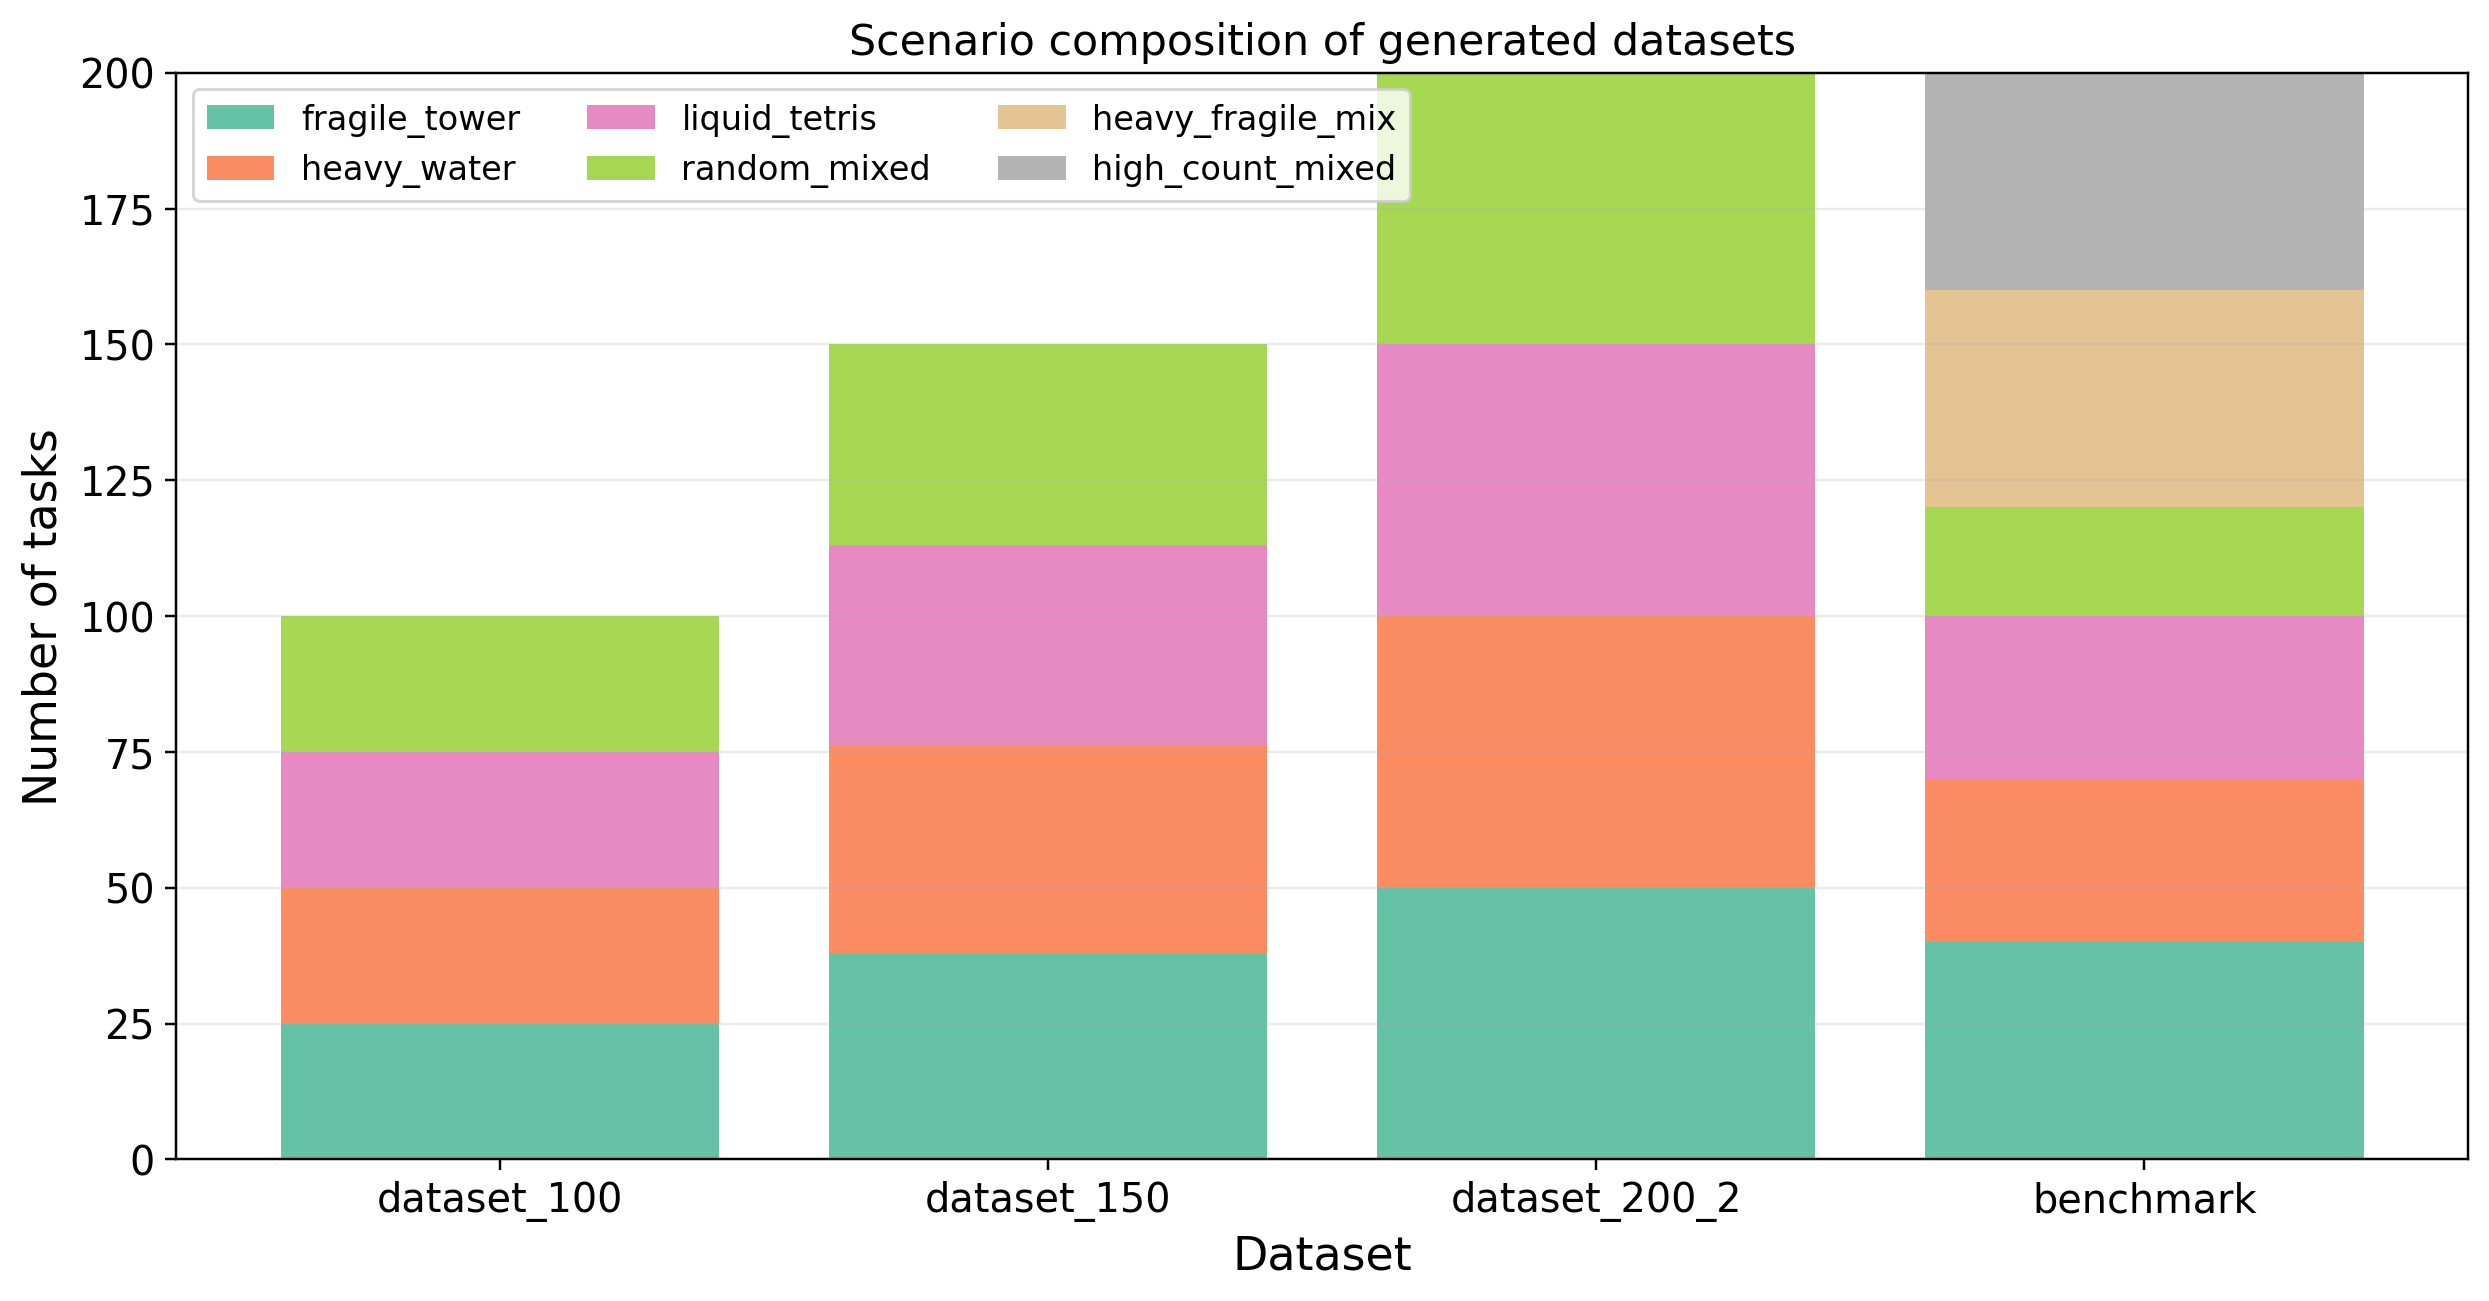
\includegraphics[width=0.95\textwidth]{dataset_composition.png}
\caption{Сценарный состав сгенерированных наборов задач}
\label{fig:dataset-composition}
\end{figure}

\subsection{\centering{Валидатор и единая оценка}}

Файл \code{validator.py} является центральным элементом экспериментальной методологии. Он не зависит от конкретного решателя и выполняет одинаковые проверки для всех ответов. Сначала валидатор восстанавливает геометрию размещенных коробов по координатам и размерам, затем проверяет anti-cheat условие: фактические размеры должны быть перестановкой исходных.

После этого последовательно проверяются масса, границы паллеты, ограничение \code{strict\_upright}, трехмерные пересечения и опора. Только валидные решения получают метрики. Такой подход исключает ситуацию, когда один метод оценивается по более мягким правилам, чем другой.

\subsection{\centering{Greedy-решатель}}

Файл \code{solvers/greedy\_algorithm.py} реализует последовательный алгоритм на extreme points. Количество каждого SKU разворачивается в список отдельных экземпляров. Затем объекты сортируются по объему, причем хрупкие и нештабелируемые товары получают специальный приоритет, чтобы уменьшить риск плохой структуры укладки.

Для каждого объекта перебираются допустимые повороты. Функция \code{get\_rotations} возвращает ориентации из множества \code{LWH}, \code{LHW}, \code{WLH}, \code{WHL}, \code{HLW}, \code{HWL}; для \code{strict\_upright} остаются только повороты с исходной высотой. Проверки пересечений, опоры и хрупкости ускорены пространственной сеткой \code{PlacedGrid}, которая ограничивает число уже размещенных коробов, участвующих в геометрических проверках.

Преимущество greedy -- скорость и простота. На всех сохраненных single-pallet наборах средний временной балл равен 1.0. Недостаток -- невозможность перестроить ранние решения, что особенно заметно на \code{dataset\_benchmark.json}: средний item coverage снижается до 0.4906.

\subsection{\centering{MaxRects-решатель}}

Файл \code{solvers/solve\_conditions.py} реализует послойный подход. Для каждого слоя выбирается высота-кандидат, после чего основания коробов упаковываются двумерным MaxRects-подобным алгоритмом. Метод сортирует товары по массе и объему, пытается заполнить слой, затем переходит к следующей высоте.

Этот решатель очень быстр: среднее время на контрольном наборе составляет около 52 мс. Он достигает высокой утилизации объема, но заметно проигрывает по хрупкости. Такое поведение объясняется тем, что послойная плотность и сортировка по весу не всегда согласуются с правилом размещения хрупких товаров верхним слоем.

\subsection{\centering{LNS-решатель}}

Файл \code{solvers/lns\_solver.py} содержит наиболее сильный решатель проекта. Его pipeline показан на рисунке~\ref{fig:lns-pipeline}.

\begin{figure}[H]
\centering
\resizebox{0.98\textwidth}{!}{%
\begin{tikzpicture}[
  node distance=9mm and 10mm,
  processnode/.style={draw, rounded corners=2pt, fill=blue!7, minimum width=31mm,
    minimum height=10mm, align=center, font=\small},
  phase/.style={draw, rounded corners=2pt, fill=green!9, minimum width=31mm,
    minimum height=10mm, align=center, font=\small},
  decide/.style={draw, diamond, aspect=2.1, fill=orange!12,
    align=center, font=\small, inner sep=1.5pt},
  arrow/.style={-{Latex[length=2.2mm]}, thick},
  loop/.style={-{Latex[length=2.2mm]}, thick, dashed}
]
\node[processnode] (input) {Входная\\задача};
\node[phase, right=of input] (start) {Построение\\начального решения};
\node[phase, right=of start] (destroy) {Destroy:\\удаление части\\коробов};
\node[phase, right=of destroy] (stabilize) {Стабилизация\\опоры};
\node[phase, right=of stabilize] (repair) {Repair:\\beam search};

\node[phase, below=11mm of repair] (evaluate) {Оценка\\кандидата};
\node[phase, left=of evaluate] (accept) {Принятие\\по score/SA};
\node[processnode, left=of accept] (current) {Обновление\\текущего решения};
\node[processnode, left=of current] (stop) {Проверка\\бюджета времени};
\node[processnode, left=of stop] (output) {Ответ JSON\\и метрики};
\node[processnode, below=8mm of accept] (best) {Обновление\\лучшего решения};

\draw[arrow] (input) -- (start);
\draw[arrow] (start) -- (destroy);
\draw[arrow] (destroy) -- (stabilize);
\draw[arrow] (stabilize) -- (repair);
\draw[arrow] (repair) -- (evaluate);
\draw[arrow] (evaluate) -- (accept);
\draw[arrow] (accept) -- (current);
\draw[loop] (accept) -- node[right, font=\footnotesize] {если лучше} (best);
\draw[loop] (best.west) to[out=180,in=-90] (output.south);
\draw[arrow] (current) -- (stop);
\draw[loop] (stop.north) to[out=90,in=-90] node[above, font=\footnotesize] {продолжить} (destroy.south);
\draw[arrow] (stop) -- node[above, font=\footnotesize] {стоп} (output);
\end{tikzpicture}%
}
\caption{Основные этапы LNS-решателя}
\label{fig:lns-pipeline}
\end{figure}

Сначала LNS строит начальное решение. В отличие от одиночного greedy-запуска, используется несколько детерминированных порядков и случайные рестарты в пределах бюджета \code{greedy\_phase\_s}. Затем запускается основной цикл destroy/repair. В реализации присутствуют destroy-эвристики:
\begin{itemize}
  \item случайное удаление размещенных коробов;
  \item удаление верхних коробов;
  \item удаление пространственного кластера;
  \item удаление коробов, связанных с нарушениями хрупкости;
  \item удаление коробов, близких по объему к непомещенным;
  \item полный рестарт;
  \item удаление малых размещенных коробов.
\end{itemize}

После разрушения вызывается стабилизация частичного решения: если некоторые короба потеряли достаточную опору, они также удаляются. Этап repair основан на beam search. Для частичных состояний применяется оценка
\begin{equation}
\mathrm{partial\_score}=0.50U_{\mathrm{vol}}+0.30C_{\mathrm{items}}-0.005n_{\mathrm{frag\_viol}},
\label{eq:partial}
\end{equation}
которая ориентирует восстановление на объем, покрытие и умеренный штраф за потенциальные нарушения хрупкости.

Ключевые параметры LNS приведены в таблице~\ref{tab:lns-params}.

\begin{table}[H]
\caption{Основные параметры LNS-конфигурации}
\label{tab:lns-params}
\centering
\small
\begin{tabular}{lcl}
\toprule
\textbf{Параметр} & \textbf{Значение} & \textbf{Назначение} \\
\midrule
\code{time\_budget\_s} & 4.8 & общий бюджет времени \\
\code{greedy\_phase\_s} & 1.5 & стартовая greedy-фаза \\
\code{destroy\_k\_fraction} & 0.15 & доля удаляемых коробов \\
\code{destroy\_k\_min/max} & 3 / 15 & границы размера разрушения \\
\code{beam\_width} & 8 & ширина beam search \\
\code{repair\_queue\_limit} & 50 & максимальная очередь восстановления \\
\code{repair\_restarts} & 2 & дополнительные repair-рестарты \\
\code{early\_stop\_patience} & 25 & остановка при отсутствии улучшений \\
\code{ils\_kicks} & 5 & число ILS-перезапусков \\
\code{sa\_initial\_temp} & 0.015 & начальная температура simulated annealing \\
\code{sa\_cooling\_rate} & 0.92 & скорость охлаждения \\
\bottomrule
\end{tabular}
\end{table}

\subsection{\centering{GAN+GA-решатель}}

Файл \code{solvers/gan\_ga\_solver.py} реализует гибрид генетического алгоритма и простой генеративно-состязательной модели. Хромосома состоит из перестановки объектов и списка выборов ориентаций. Декодер строит укладку greedy-методом с ограниченным числом extreme points.

Генетическая часть использует турнирный отбор, order crossover, скрещивание ориентаций и мутации перестановки. GAN-компонента реализована на NumPy: генератор создает приоритеты объектов, преобразуемые в перестановку, а дискриминатор оценивает похожесть решения на элитные особи. Эта оценка добавляется к fitness с малым коэффициентом.

Метод интересен как ML-ориентированная альтернатива, но в текущих экспериментах уступает LNS по среднему score на общих наборах. При этом GAN+GA сохраняет высокий fragility score и демонстрирует конкурентную утилизацию объема.

\subsection{\centering{Визуализация}}

Каталог \code{vizualizator} содержит средства просмотра результатов. Визуализатор читает входной JSON и JSON с размещениями, строит трехмерное представление паллеты и позволяет анализировать слои. Для дипломной работы на основе сохраненного результата LNS построен пример укладки на рисунке~\ref{fig:example-packing}.

\begin{figure}[H]
\centering
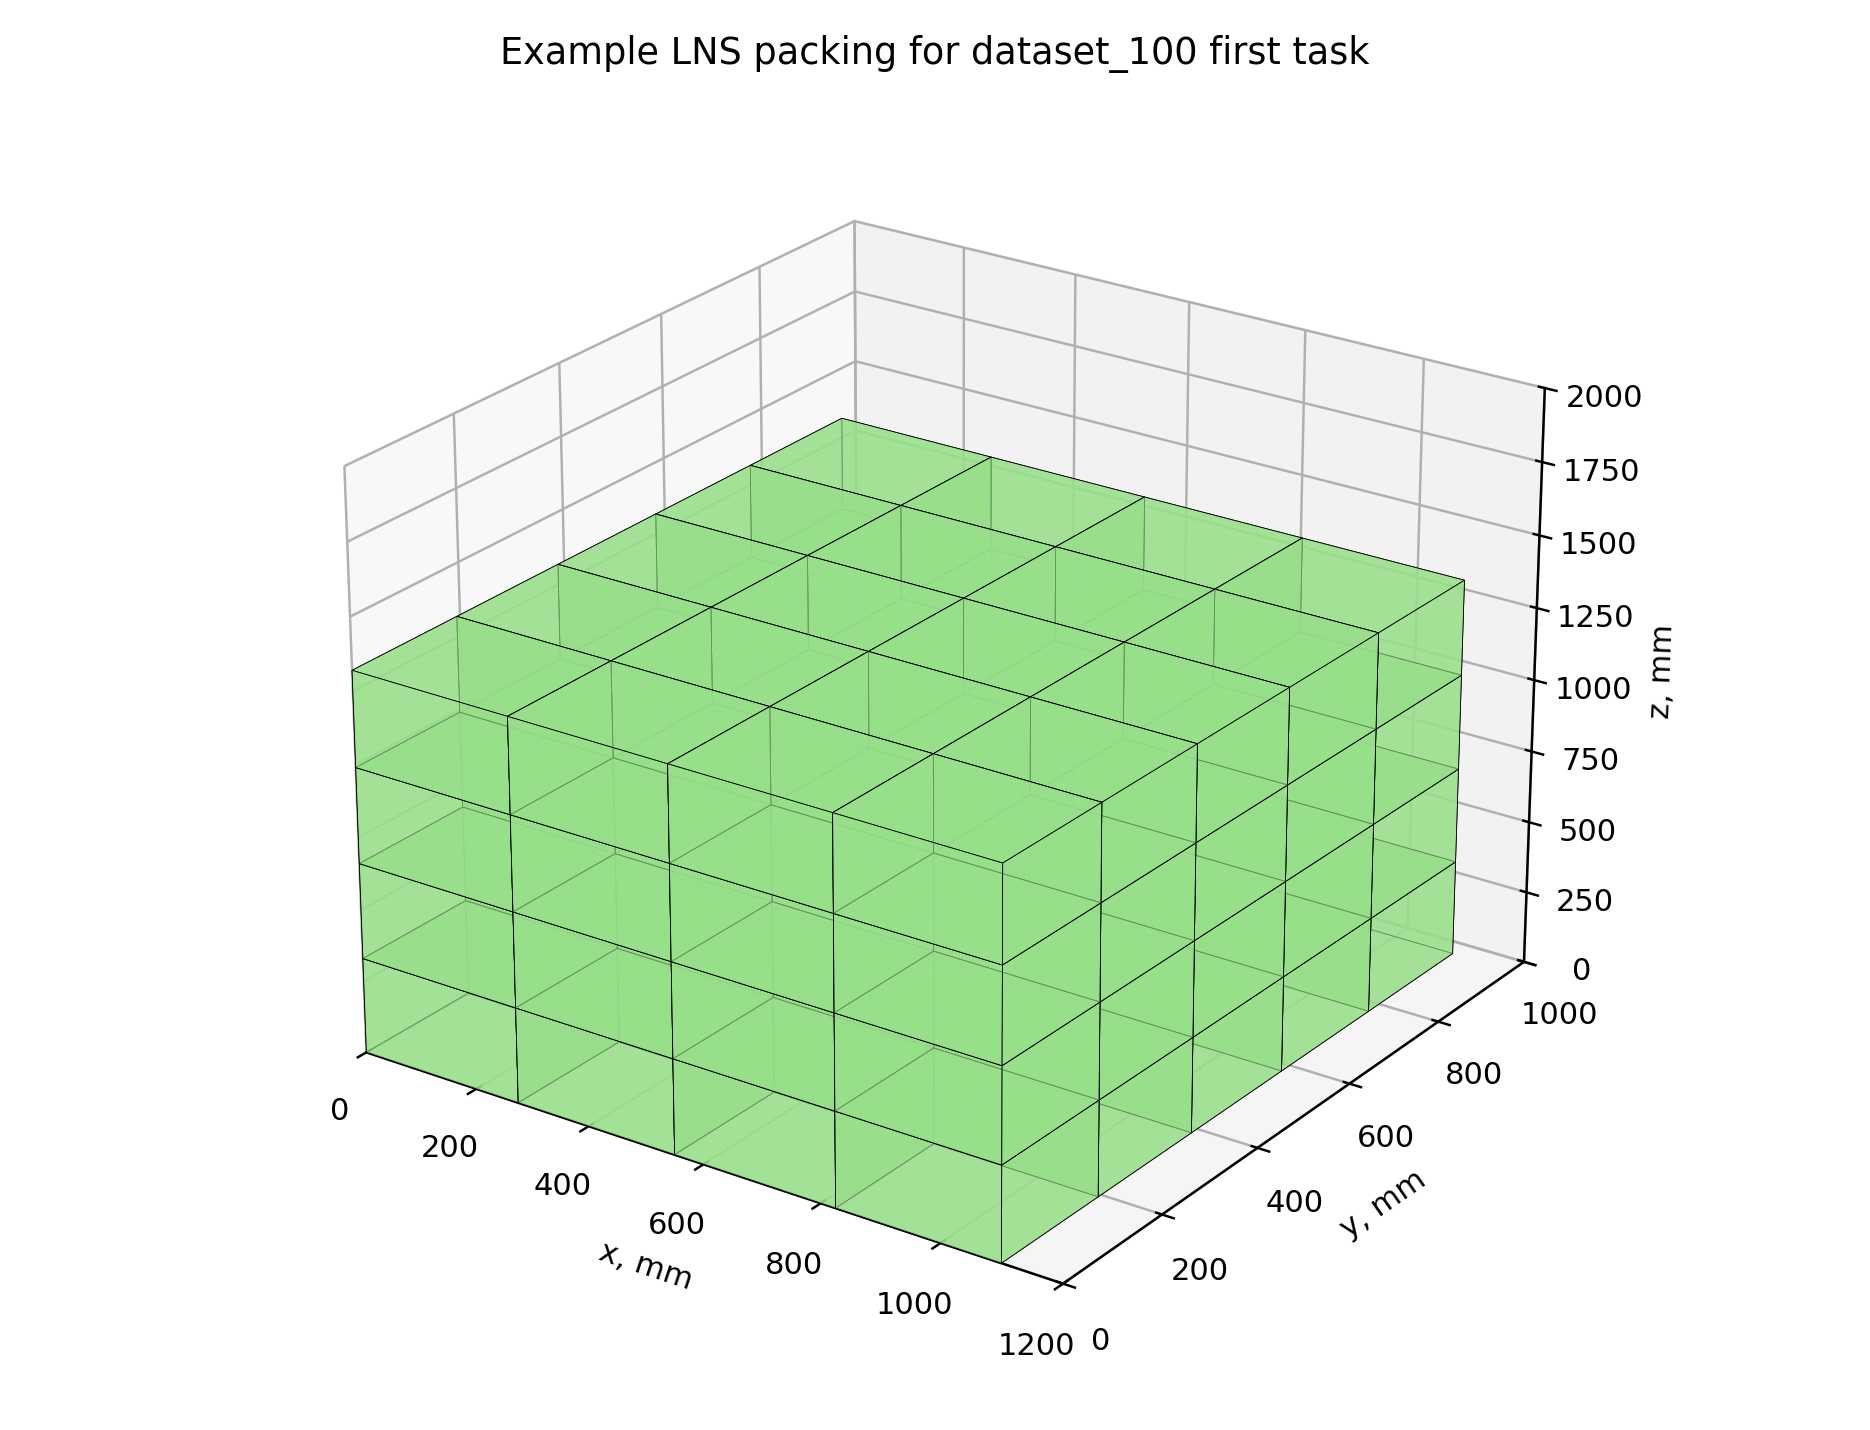
\includegraphics[width=0.80\textwidth]{example_lns_packing.png}
\caption{Пример укладки, построенной LNS для первой задачи \code{dataset\_100.json}}
\label{fig:example-packing}
\end{figure}

\subsection{\centering{Выводы по разделу}}

Проект представляет собой не отдельный алгоритм, а полноценный исследовательский стенд. Его сильная сторона -- единый формат данных, общий валидатор и сохраненные результаты для нескольких решателей. На уровне реализации наиболее развитым методом является LNS: он использует greedy как стартовую эвристику, но дополняет ее разрушением и восстановлением фрагментов решения, адаптивными эвристиками и simulated annealing.

\clearpage
\section[\MakeUppercase{Эксперименты, метрики и анализ результатов}]{\centering\MakeUppercase{Эксперименты, метрики и анализ результатов}}

\subsection{\centering{Методика эксперимента}}

Экспериментальная часть основана на уже сохраненных результатах из каталога \code{results}. Для каждого решателя и датасета в JSON-файлах содержатся ответы по отдельным задачам, рассчитанные метрики и время решения. Такой подход выбран намеренно: он исключает повторную случайную генерацию результатов и позволяет опираться на фактические данные проекта.

При сравнении эвристических методов особенно важно использовать единый протокол оценки. Если один алгоритм проверяется более мягким валидатором, а другой -- более строгим, итоговое сравнение теряет смысл. В данном проекте все результаты проходят через \code{validator.py}, поэтому различия в score отражают именно свойства построенных укладок. Это также упрощает воспроизводимость: любой сохраненный JSON-ответ можно повторно проверить тем же валидатором и получить те же компоненты метрики.

Сохраненные результаты рассматриваются как экспериментальная выборка, а не как единичные демонстрационные примеры. Каждый датасет содержит множество задач с разным составом товаров, поэтому средние значения позволяют оценивать устойчивость метода к изменению входных данных. При этом отдельные наборы отличаются сложностью: \code{dataset\_benchmark.json} содержит больше объектов в задаче и более разнообразный сценарный состав, поэтому он используется как наиболее показательный контрольный набор.

В основном сравнении используются четыре single-pallet метода:
\begin{itemize}
  \item \code{greedy\_algorithm};
  \item \code{conditions} -- MaxRects-подобный послойный решатель;
  \item \code{gan\_ga\_solver};
  \item \code{lns\_solver}.
\end{itemize}

Общими для всех четырех решателей являются три набора: \code{dataset\_100.json}, \code{dataset\_200\_2.json} и \code{dataset\_benchmark.json}. Для GAN+GA дополнительно есть результат на \code{dataset\_150.json}, но он не используется в основном ранжировании, чтобы сравнение было симметричным.

Симметричность сравнения важна из-за того, что итоговый score усредняется по задачам внутри набора. Если включить датасет, на котором присутствует только один решатель, средний результат нельзя будет напрямую сопоставлять с остальными методами. Поэтому дополнительный результат GAN+GA полезен для анализа поведения метода, но не должен менять основную таблицу ранжирования.

\subsection{\centering{Сводные результаты}}

Средний итоговый score на общих наборах приведен в таблице~\ref{tab:score-main} и на рис.~\ref{fig:all-score}.

\begin{table}[H]
\caption{Средний итоговый score на общих наборах}
\label{tab:score-main}
\centering
\small
\begin{tabular}{|l|c|c|c|}
\hline
\textbf{Метод} & \textbf{\code{dataset\_100}} & \textbf{\code{dataset\_200\_2}} & \textbf{\code{dataset\_benchmark}} \\
\hline
Greedy & 0.6842 & 0.7120 & 0.6549 \\ \hline
MaxRects & 0.7104 & 0.7117 & 0.7124 \\ \hline
GAN+GA & 0.7012 & 0.7327 & 0.7161 \\ \hline
LNS & \textbf{0.7111} & \textbf{0.7434} & \textbf{0.7298} \\ \hline
\end{tabular}
\end{table}

\begin{figure}[H]
\centering
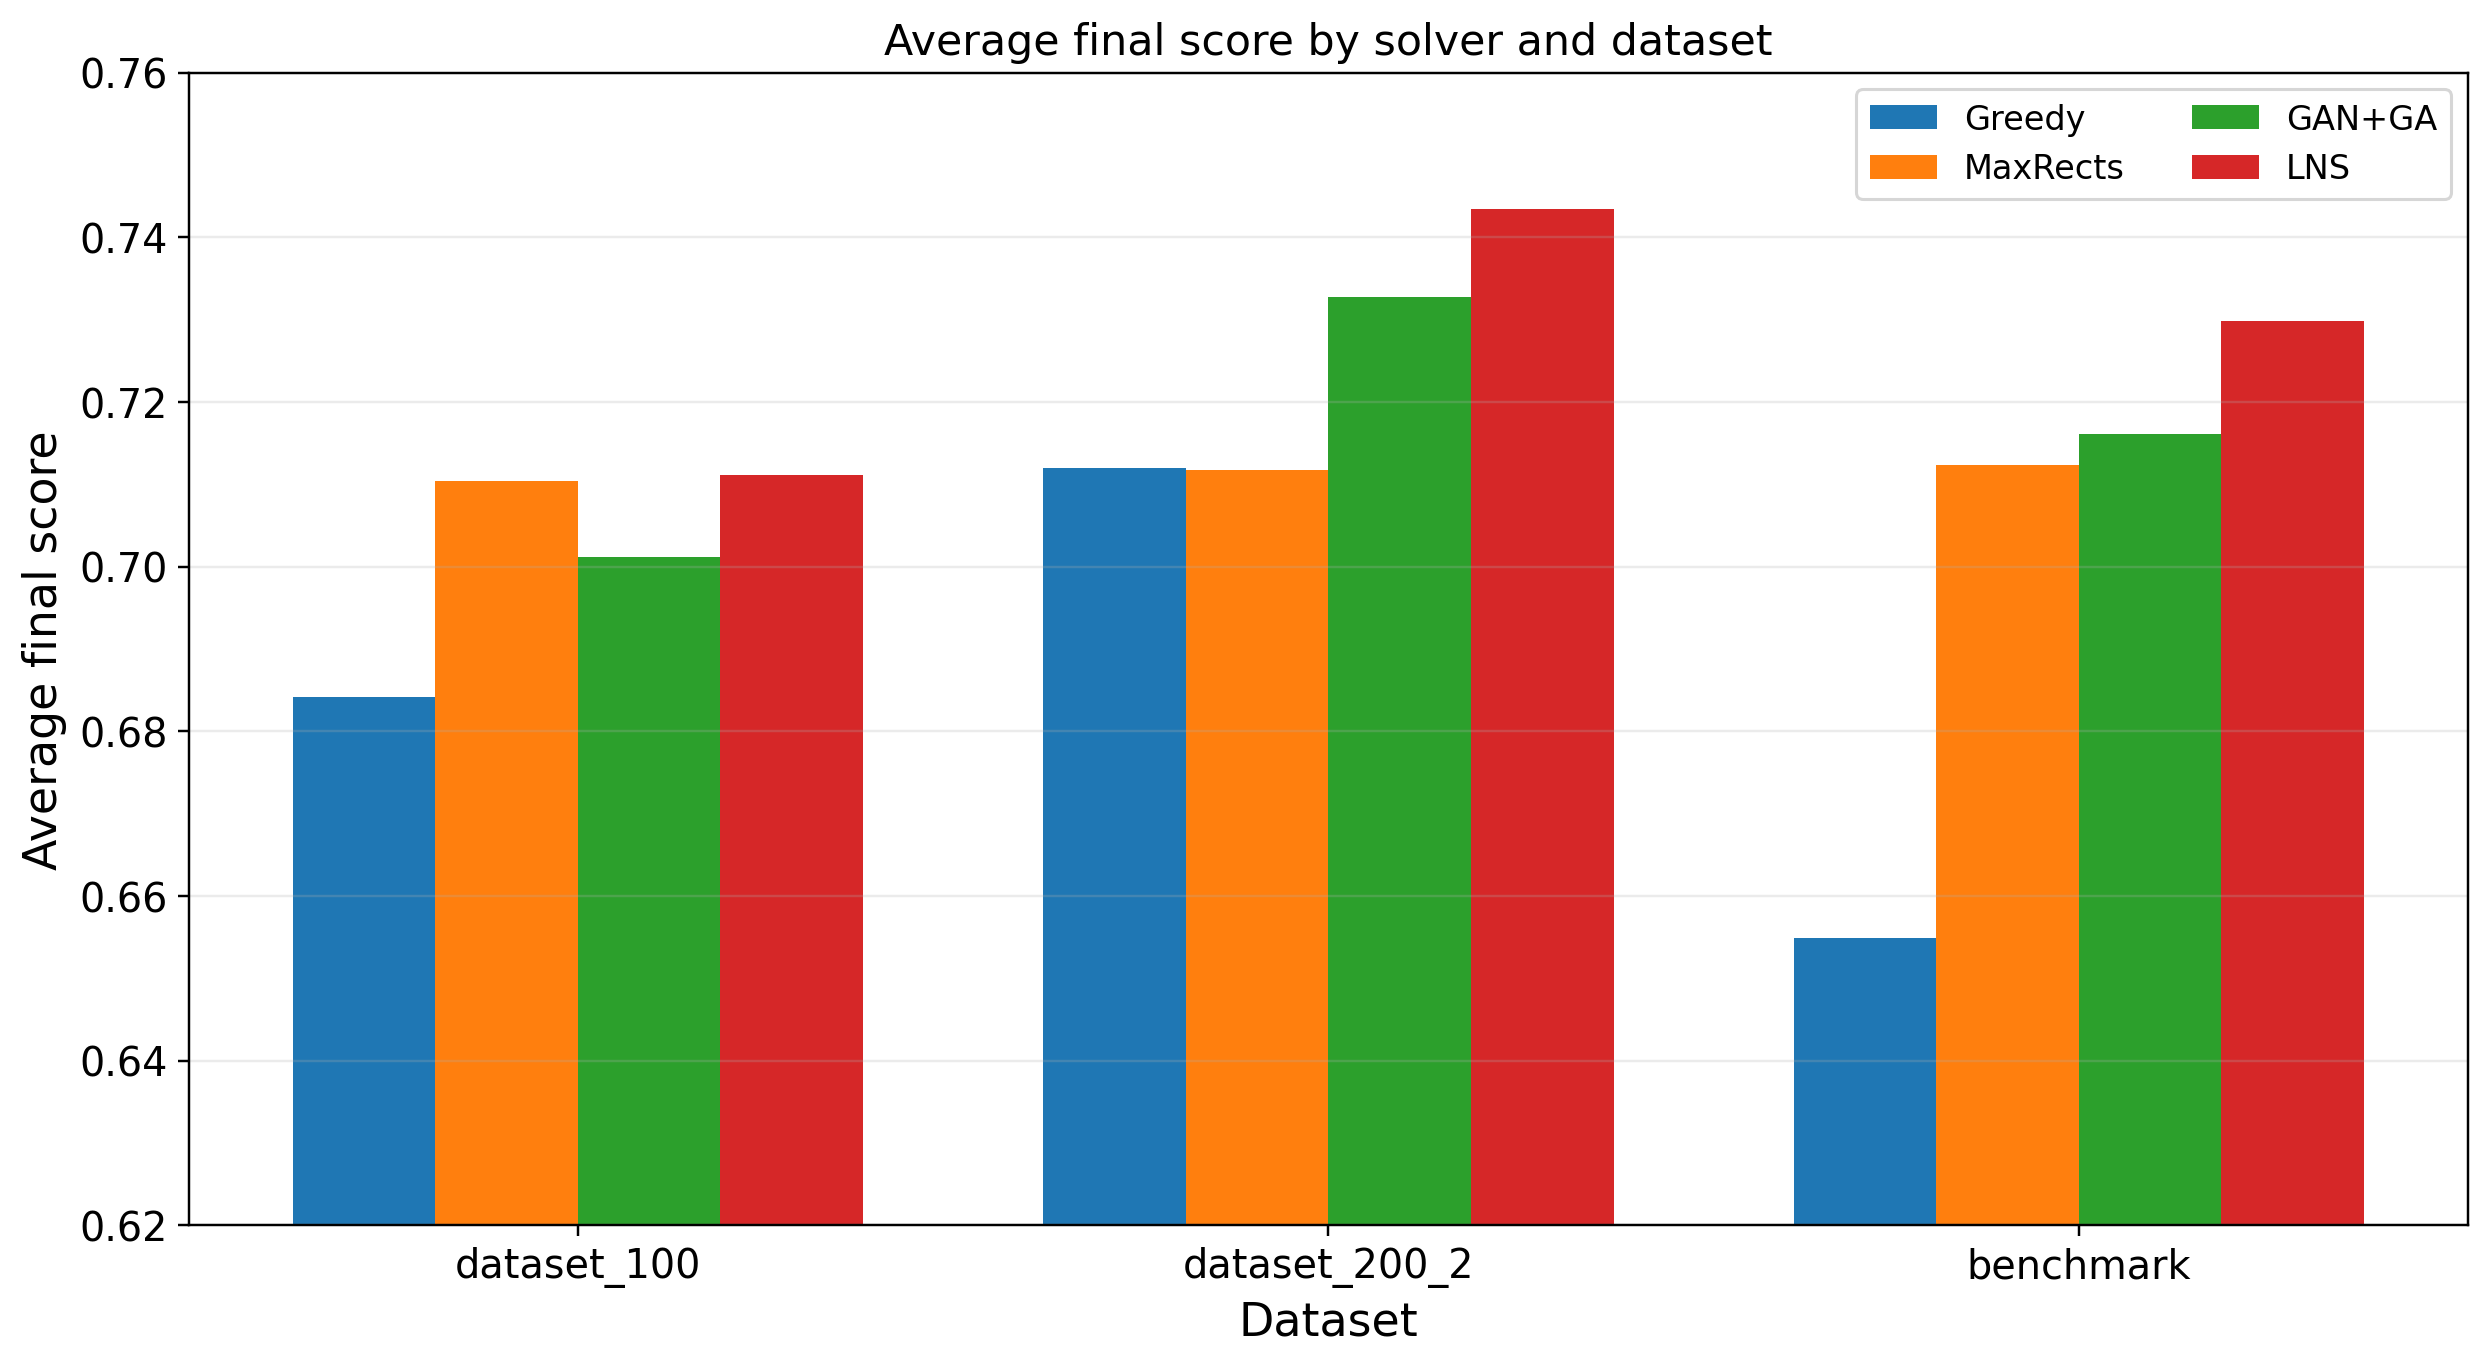
\includegraphics[width=0.97\textwidth]{all_solvers_score.png}
\caption{Средний итоговый score по решателям и датасетам}
\label{fig:all-score}
\end{figure}

LNS показывает лучший результат на всех трех общих наборах. На \code{dataset\_100.json} его преимущество над MaxRects минимально, что объясняется меньшей сложностью задач: быстрый послойный метод уже строит достаточно сильные решения. На \code{dataset\_200\_2.json} LNS заметно обгоняет остальные методы за счет лучшей полноты размещения. На \code{dataset\_benchmark.json}, где среднее число объектов выше и состав сценариев шире, преимущество LNS сохраняется.

Интерпретация этой таблицы показывает, что выигрыш LNS не является случайным эффектом одного датасета. Метод не всегда максимизирует отдельную компоненту, но стабильно удерживает высокий итоговый баланс. Для практической паллетизации такое поведение предпочтительнее, чем резкий выигрыш по одной характеристике при сильном проигрыше по другой. Например, алгоритм с максимальной утилизацией объема может оказаться менее полезным, если он часто размещает тяжелые товары над хрупкими или оставляет большую долю заказа вне паллеты.

Также важно учитывать, что различие между методами зависит от сложности набора. На простых задачах сильный baseline может быть близок к LNS, потому что пространство хороших решений достаточно широкое. На более насыщенных задачах ранние ошибки greedy и послойных методов становятся дороже: один неудачно выбранный нижний слой ограничивает все последующие уровни. В этих случаях возможность разрушить и восстановить часть укладки дает LNS преимущество.

\subsection{\centering{Компоненты метрики}}

Для интерпретации результатов рассмотрим компоненты score на контрольном наборе \code{dataset\_benchmark.json}. Данные приведены в таблице~\ref{tab:components-benchmark} и на рис.~\ref{fig:components}.

\begin{table}[H]
\caption{Компоненты метрики на \code{dataset\_benchmark.json}}
\label{tab:components-benchmark}
\centering
\small
\begin{tabular}{|l|c|c|c|c|c|}
\hline
\textbf{Метод} & \textbf{Score} & \textbf{Vol.} & \textbf{Coverage} & \textbf{Fragility} & \textbf{Time} \\
\hline
Greedy & 0.6549 & 0.6155 & 0.4906 & 1.0000 & 1.0000 \\ \hline
MaxRects & 0.7124 & \textbf{0.7513} & \textbf{0.6160} & 0.5198 & 1.0000 \\ \hline
GAN+GA & 0.7161 & 0.7156 & 0.5540 & \textbf{1.0000} & 0.9205 \\ \hline
LNS & \textbf{0.7298} & 0.7172 & 0.6036 & 0.9833 & 0.9175 \\ \hline
\end{tabular}
\end{table}

\begin{figure}[H]
\centering
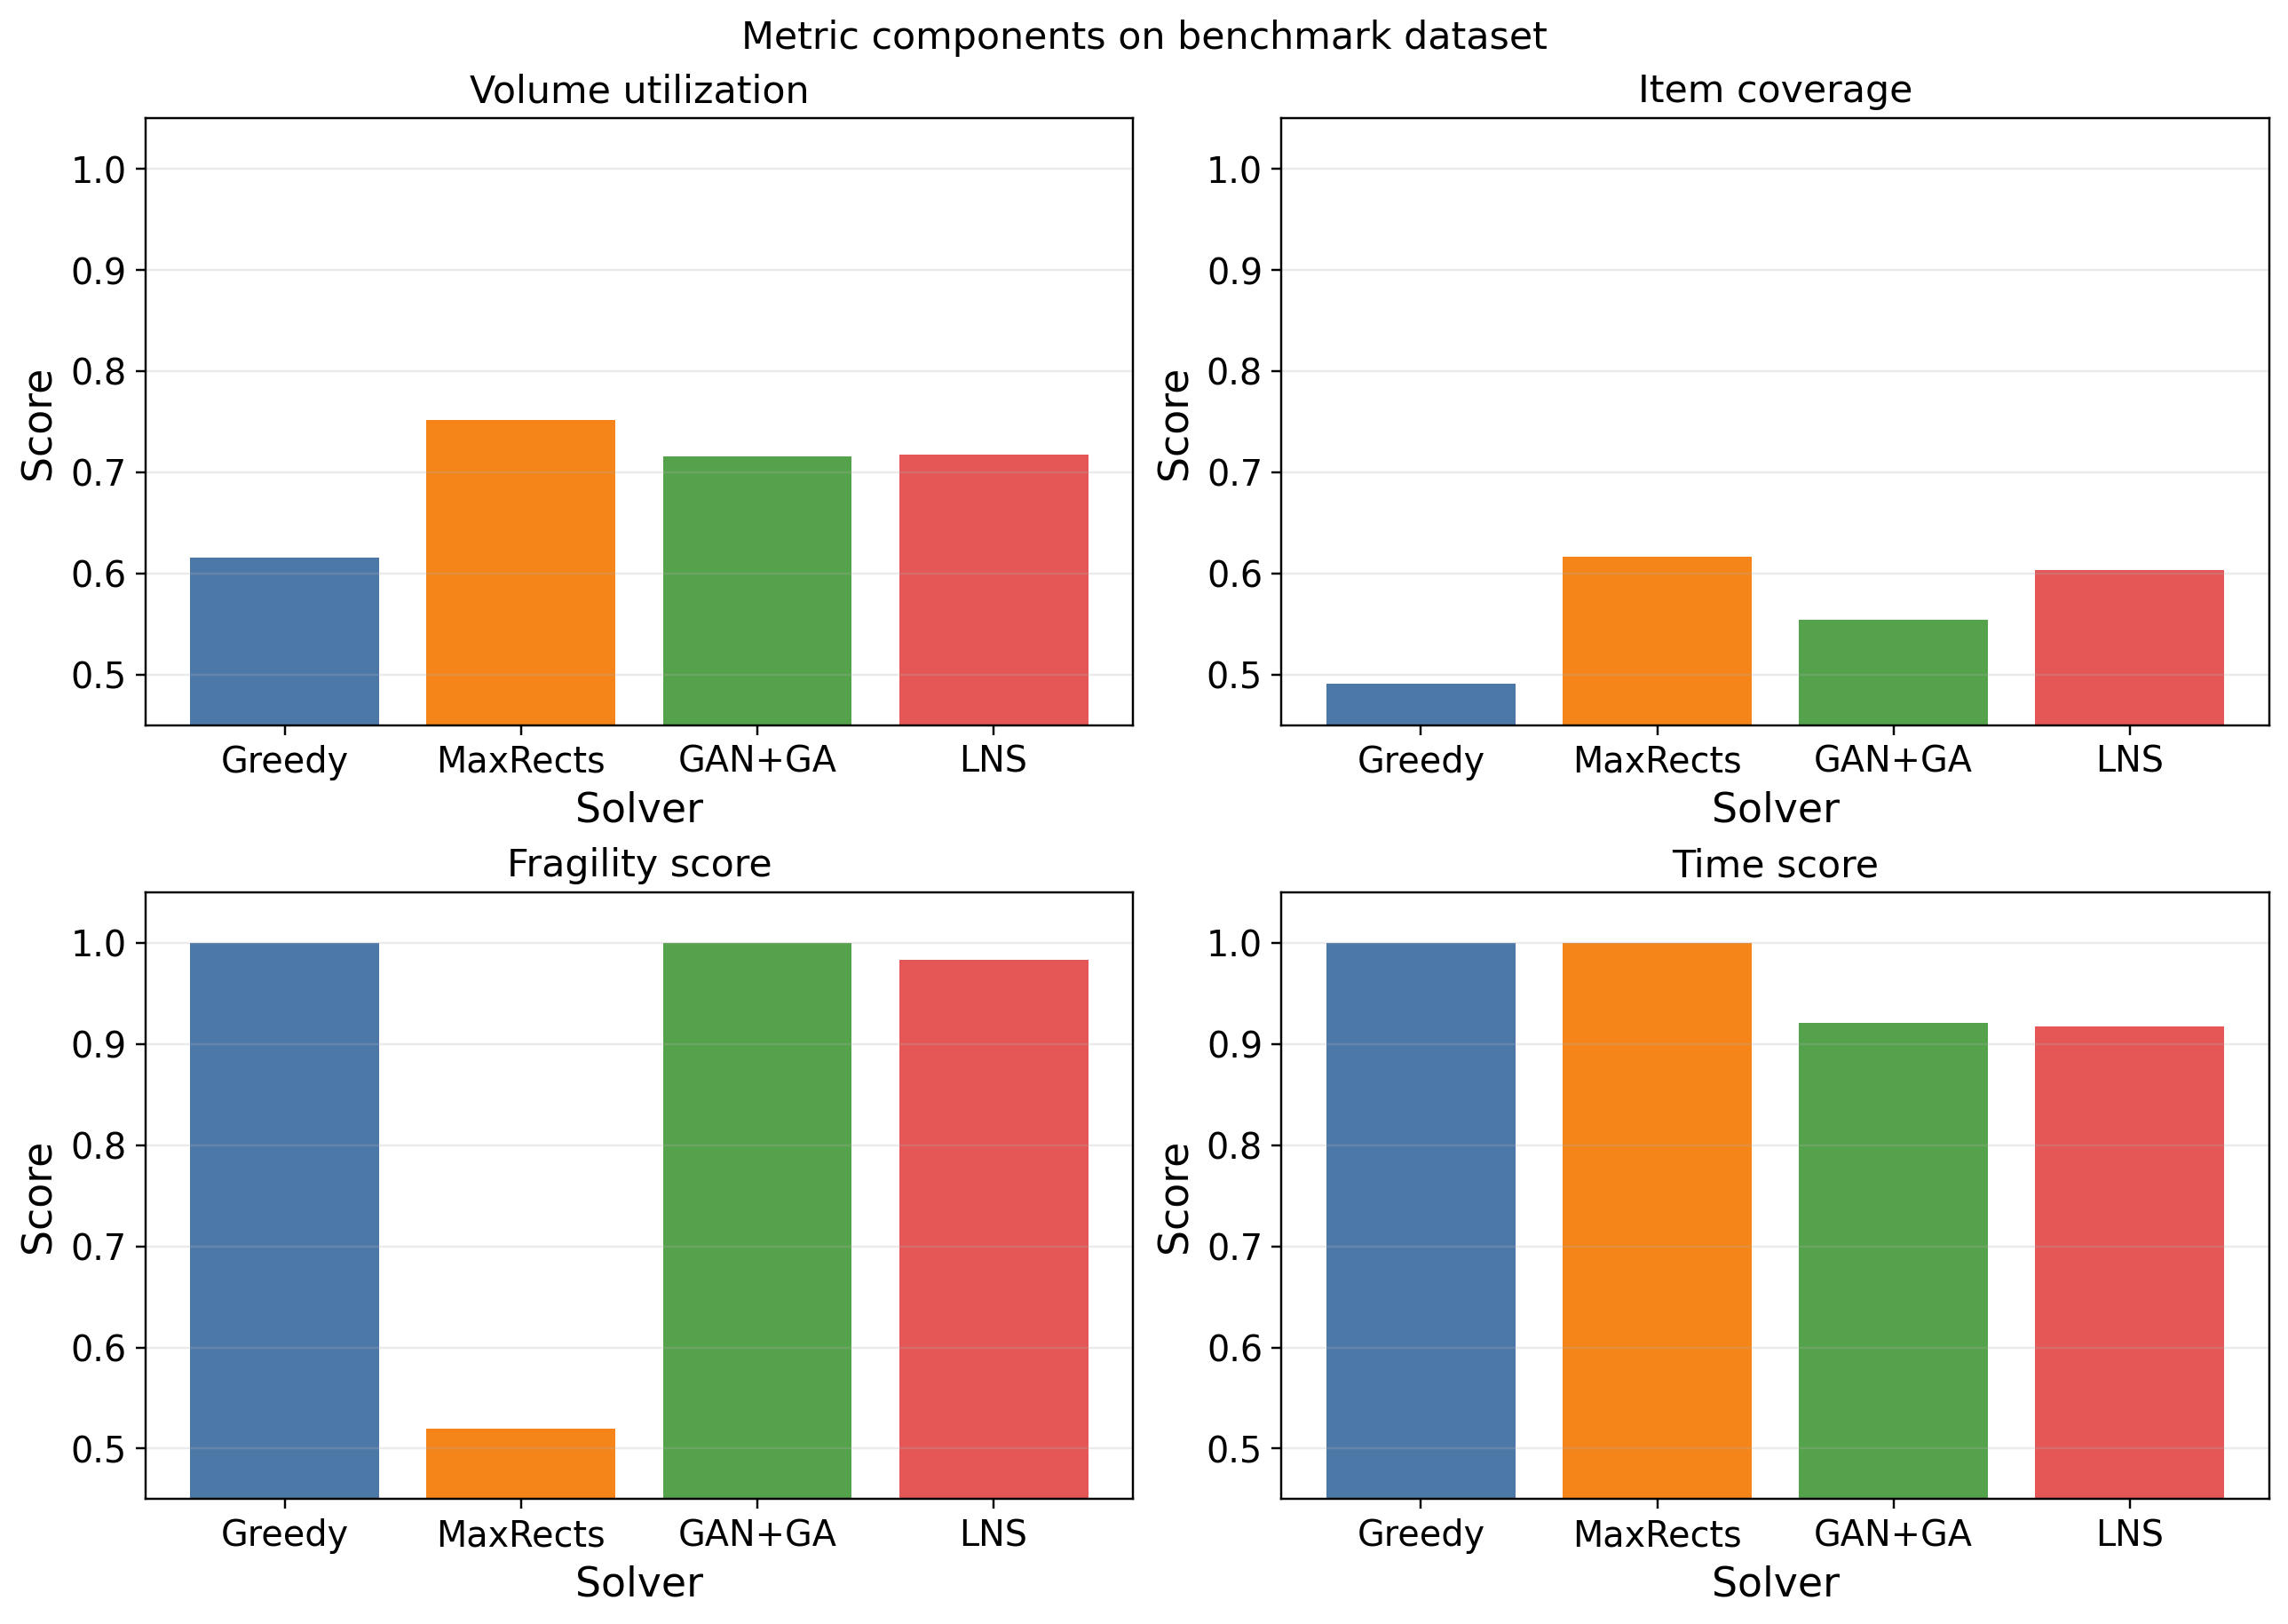
\includegraphics[width=0.98\textwidth]{benchmark_components.png}
\caption{Компоненты score на контрольном наборе}
\label{fig:components}
\end{figure}

Greedy сохраняет идеальные значения по хрупкости и времени, но значительно уступает по покрытию заказа. MaxRects достигает максимальной утилизации объема и максимального покрытия на контрольном наборе, однако теряет почти половину балла за хрупкость. GAN+GA хорошо соблюдает хрупкость и заметно улучшает объем по сравнению с greedy, но уступает LNS по покрытию.

LNS не максимизирует отдельную компоненту любой ценой. Его сила заключается в балансе: утилизация объема близка к GAN+GA, покрытие близко к MaxRects, хрупкость остается высокой, а временной балл остается приемлемым. Именно этот баланс дает лучший итоговый score.

Компонентный анализ показывает, почему итоговая метрика полезнее одного показателя заполнения объема. MaxRects достигает наибольшей утилизации и покрытия на контрольном наборе, но сильная потеря по хрупкости снижает итоговую оценку. Greedy, наоборот, сохраняет идеальную хрупкость и скорость, но слишком часто оставляет часть заказа неразмещенной. LNS занимает промежуточное положение по отдельным компонентам, но именно поэтому оказывается наиболее устойчивым по суммарному критерию.

Такой результат согласуется с логикой выбранной метрики. В реальной задаче паллетизации нельзя оптимизировать только геометрию, игнорируя свойства товара. Укладка должна быть плотной, но не должна создавать чрезмерный риск повреждения, а время расчета должно оставаться приемлемым для использования в операционном контуре. Поэтому метод, который немного уступает по объему, но лучше соблюдает остальные требования, может получать более высокий итоговый score.

\subsection{\centering{Время выполнения}}

Среднее фактическое время решения приведено в таблице~\ref{tab:runtime}. Все методы на основных наборах остаются в пределах практически приемлемого времени. Greedy и MaxRects работают быстрее всех, LNS и GAN+GA тратят около секунды на контрольном наборе.

\begin{table}[H]
\caption{Среднее время решения, мс}
\label{tab:runtime}
\centering
\small
\begin{tabular}{|l|c|c|c|}
\hline
\textbf{Метод} & \textbf{\code{dataset\_100}} & \textbf{\code{dataset\_200\_2}} & \textbf{\code{dataset\_benchmark}} \\
\hline
Greedy & 114.8 & 118.5 & 139.0 \\ \hline
MaxRects & 15.1 & 15.6 & 52.0 \\ \hline
GAN+GA & 795.3 & 770.4 & 1080.6 \\ \hline
LNS & 474.3 & 523.6 & 1062.6 \\ \hline
\end{tabular}
\end{table}

Увеличение времени LNS оправдано ростом основных компонент качества. На контрольном наборе LNS теряет часть временного балла, но выигрывает по итоговой оценке. Это соответствует назначению метаэвристики: использовать дополнительное время не на случайное усложнение, а на улучшение структуры укладки.

С точки зрения прикладного применения абсолютное время LNS остается небольшим: на контрольном наборе оно измеряется примерно одной секундой. Для пакетного планирования паллет или предварительного расчета заказов такой уровень затрат обычно приемлем. Если же система должна работать строго в интерактивном режиме, можно уменьшить бюджет LNS и использовать greedy или MaxRects как быстрый fallback, сохраняя единый формат ответа и валидации.

При этом время выполнения следует рассматривать вместе с размером задачи и требуемым качеством ответа. Для небольших заказов выигрыш сложной метаэвристики может быть несущественным, поскольку быстрый решатель уже находит близкое по качеству решение. Для насыщенных заказов с большим числом коробов дополнительная секунда расчета может окупаться за счет более полного размещения и меньшего числа переносов товара на следующую паллету. Поэтому практическая система может выбирать метод адаптивно: запускать быстрый baseline для простых случаев и включать LNS для задач, где требуется улучшить плотность или покрытие.

\subsection{\centering{Сравнение LNS и Greedy}}

В рамках НИР отдельно исследовался LNS как развитие базового greedy. Для этой пары доступны графики, построенные из сохраненных результатов. На рис.~\ref{fig:lns-greedy-score} показано, что LNS стабильно превосходит greedy по среднему score на трех наборах.

\begin{figure}[H]
\centering

\includegraphics[width=0.85\textwidth]{lns_vs_greedy_score.png}
\caption{Сравнение среднего score для LNS и greedy}
\label{fig:lns-greedy-score}
\end{figure}

Компонентное сравнение на рис.~\ref{fig:lns-greedy-metrics} показывает, что главный вклад LNS дает по утилизации объема и покрытию заказа. Небольшое ухудшение по времени и хрупкости не перекрывает этот выигрыш.

\begin{figure}[H]
\centering
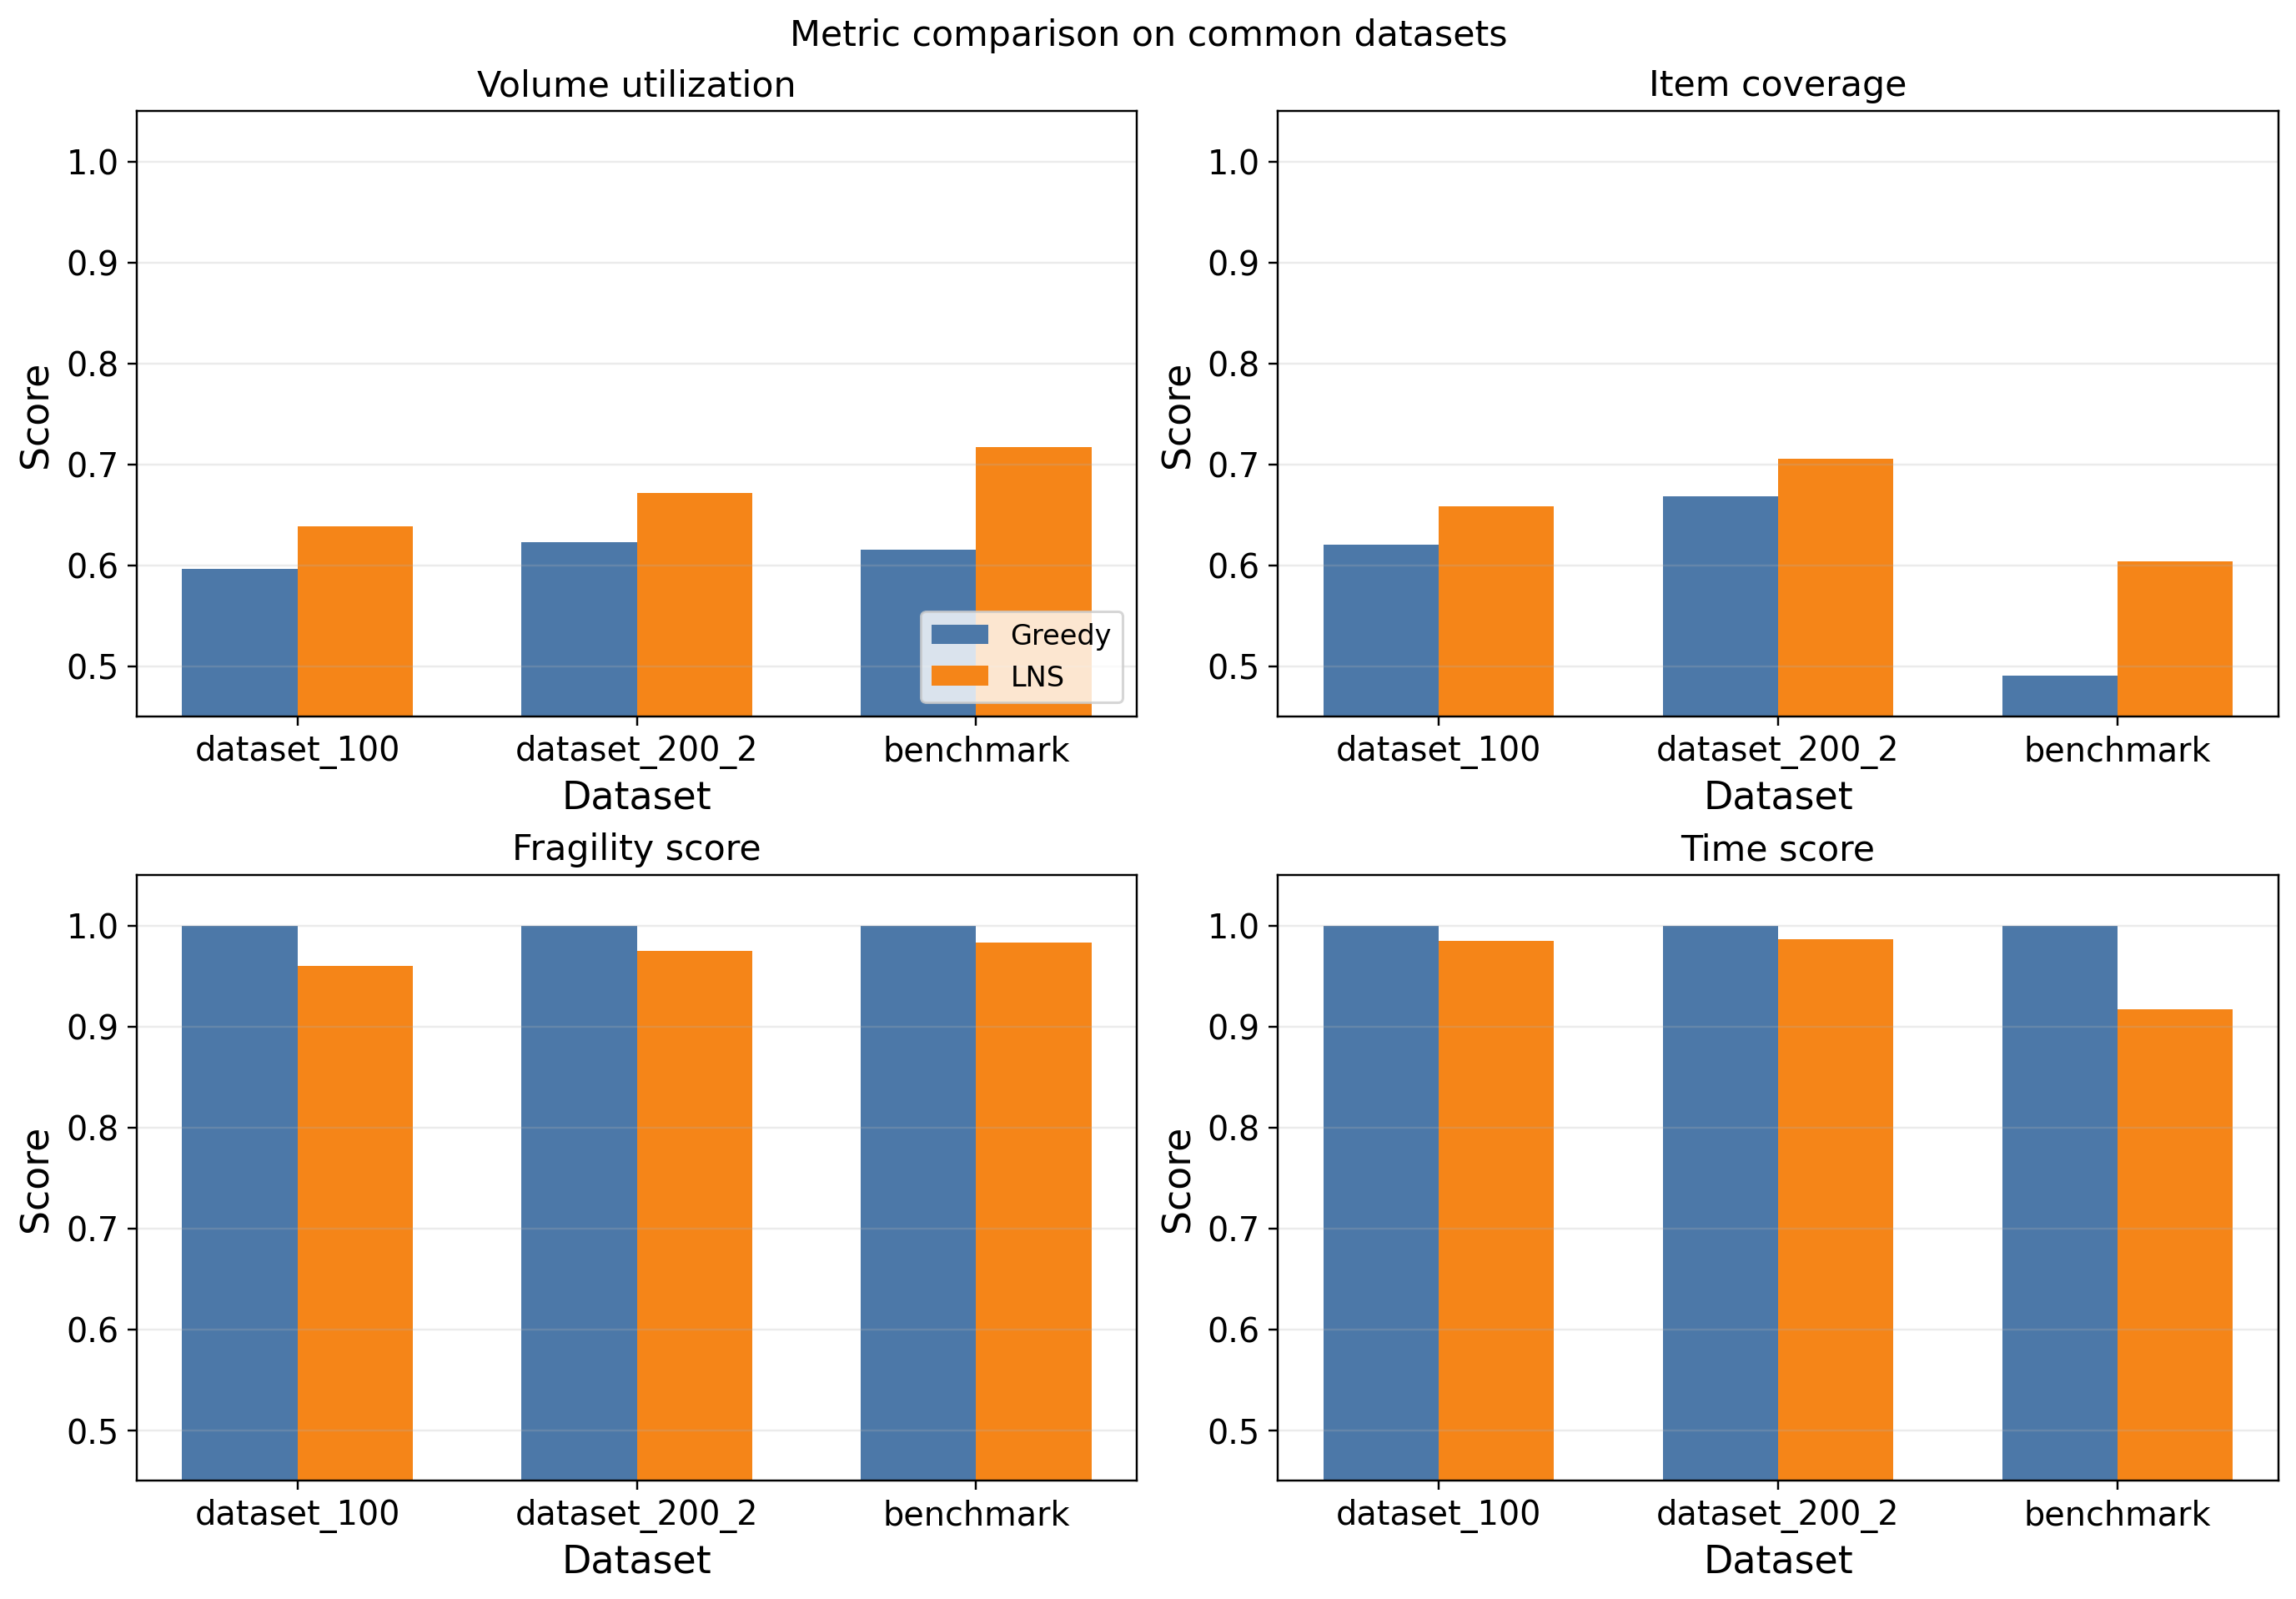
\includegraphics[width=0.95\textwidth]{lns_vs_greedy_metrics.png}
\caption{Сравнение компонент метрики для LNS и greedy}
\label{fig:lns-greedy-metrics}
\end{figure}

\subsection{\centering{Сравнение с brute force на малых задачах}}

Каталог \code{brute\_force\_vs\_algo} содержит отдельные эксперименты для малых и средних наборов. Их цель -- оценить поведение LNS рядом с более полным поиском. Результаты приведены в таблице~\ref{tab:brute}.

\begin{table}[H]
\caption{Сравнение brute force и LNS на специальных наборах}
\label{tab:brute}
\centering
\small
\begin{tabular}{|l|l|r|r|r|}
\hline
\textbf{Набор} & \textbf{Метод} & \textbf{Score} & \textbf{Coverage} & \textbf{Время, мс} \\
\hline
small & Brute force & 0.5563 & 0.9897 & 19.5 \\ \hline
small & LNS & \textbf{0.5602} & \textbf{1.0000} & 28.3 \\ \hline
medium & Brute force & 0.5681 & 0.9921 & 10440.7 \\ \hline
medium & LNS & \textbf{0.5780} & \textbf{1.0000} & 72.5 \\ \hline
hard & Brute force / LDS & 0.5886 & 0.9364 & 8815.0 \\ \hline
hard & LNS & \textbf{0.6501} & \textbf{1.0000} & 243.2 \\ \hline
\end{tabular}
\end{table}

На этих наборах LNS не только сопоставим с перебором, но и превосходит сохраненные результаты brute force/LDS по итоговой метрике. Важно, что для medium и hard время перебора резко возрастает, тогда как LNS остается в пределах сотен миллисекунд. Это подтверждает практическую ценность метаэвристического подхода.

\subsection{\centering{Многопаллетное расширение}}

В каталоге \code{multipallet} реализовано расширение на несколько паллет. Эта постановка ближе к реальной логистике: если весь заказ нельзя разместить на одной паллете, требуется распределить оставшиеся товары на новые паллеты. В проекте есть single-pallet и multi-pallet решения для greedy и LNS.

В рамках данной ВКР многопаллетный режим рассматривается как направление развития, поскольку основная метрика и основные benchmark-результаты сосредоточены на single-pallet постановке. Тем не менее наличие отдельного каталога \code{multipallet} показывает, что архитектура проекта допускает переход от локальной задачи плотной укладки к задаче распределения заказа между несколькими контейнерами.

Многопаллетная постановка меняет смысл оптимизации. В single-pallet варианте часть товара может остаться неразмещенной, и это отражается в компоненте покрытия. В multi-pallet режиме требуется решить, сколько паллет использовать и как распределить товары между ними. Тогда к текущим критериям добавляется стоимость дополнительной паллеты, а также могут появиться требования группировки товаров по магазинам, маршрутам или температурным зонам. Поэтому имеющееся расширение следует рассматривать как основу, которую нужно дополнить отдельной метрикой и отдельными экспериментами.

\subsection{\centering{Анализ ошибок и ограничений}}

Анализ кода и результатов позволяет выделить несколько ограничений текущей реализации.

Во-первых, модель устойчивости приближенная. Критерий 60\% опоры учитывает площадь контакта, но не анализирует центр масс, распределение давления, трение и деформации упаковки. Поэтому решение может быть валидным по формальному критерию, но требовать дополнительной инженерной проверки перед промышленным применением.

Во-вторых, синтетические данные не покрывают всего разнообразия реальных заказов. В генераторе есть полезные сценарии фуд-ритейла, но нет, например, температурных зон, запрета соседства, приоритетов выгрузки, ограничений по слоям и требований к группировке товаров по магазинам.

В-третьих, GAN+GA является облегченной исследовательской реализацией. Он использует NumPy-модель вместо полноценного обучения на большом корпусе решений. Поэтому текущие результаты не следует трактовать как окончательный предел ML-подходов к задаче.

В-четвертых, benchmark хранит средние значения, но не содержит статистического анализа устойчивости стохастических методов по нескольким независимым запускам на каждом датасете. Для LNS и GAN+GA в дальнейшем полезно оценивать дисперсию результата.

Еще одно ограничение связано с синтетической природой основной части данных. Генератор позволяет управлять сценариями и получать воспроизводимые наборы, однако реальные складские заказы могут иметь дополнительные зависимости: совместимость товарных групп, требования к последовательности выгрузки, ограничения по температуре, запрет соседства некоторых позиций и нестандартные размеры упаковок. Поэтому полученные результаты показывают качество методов в моделируемой постановке, но для промышленного внедрения их следует дополнительно проверять на реальных данных конкретной логистической системы.

Кроме того, сохраненные benchmark-результаты фиксируют итоговые средние значения, но не всегда показывают распределение ошибок по отдельным задачам. Для дальнейшего анализа полезно выделять группы экземпляров, на которых метод чаще всего проигрывает: заказы с большим числом мелких коробов, смеси тяжелых и хрупких товаров, задачи с ограниченными поворотами или случаи почти полного заполнения паллеты. Такая детализация поможет не только улучшить средний score, но и понять, какие именно ограничения требуют новых эвристик.

\subsection{\centering{Направления развития}}

Наиболее перспективные направления дальнейшей работы:
\begin{enumerate}
  \item Улучшить физическую модель устойчивости с учетом центра масс и распределения веса;
  \item Расширить генератор данных реальными бизнес-ограничениями;
  \item Добавить статистический протокол повторных запусков стохастических методов;
  \item Развить LNS за счет адаптивного выбора destroy/repair-операторов;
  \item Исследовать reinforcement learning или imitation learning для выбора порядка размещения;
  \item Развить многопаллетную постановку с метрикой минимизации числа паллет;
  \item Добавить автоматическую генерацию HTML-отчета с интерактивной 3D-визуализацией.
\end{enumerate}

\subsection{\centering{Выводы по разделу}}

Экспериментальные результаты показывают, что лучшим single-pallet методом текущего проекта является LNS. Он стабильно превосходит greedy, MaxRects и GAN+GA по среднему итоговому score на общих наборах. Причина преимущества не в максимизации одной компоненты, а в сбалансированном улучшении объема, покрытия, хрупкости и времени. Greedy остается полезным быстрым baseline, MaxRects -- сильным послойным решателем по плотности, GAN+GA -- перспективным исследовательским направлением, а brute force -- инструментом проверки малых экземпляров.

\structsection{Заключение}

В выпускной квалификационной работе была исследована задача Smart 3D Packing, представляющая собой прикладную постановку 3D Bin Packing для укладки коробов на паллету. В отличие от абстрактной геометрической задачи, рассматриваемая постановка учитывает ограничения, характерные для складской логистики: габариты паллеты, грузоподъемность, допустимые повороты, опору, хрупкость, штабелируемость и время расчета.

В ходе работы были изучены условие задачи, материалы НИР и курсовой работы, требования к оформлению ВКР, примеры прошлых дипломов и исходный код проекта. По результатам анализа восстановлен pipeline решения: генерация или загрузка JSON-датасета, запуск одного из решателей, валидация жестких ограничений, расчет метрик, сохранение результатов и визуализация укладки.

Были рассмотрены реализованные методы: greedy на основе extreme points и gravity drop, послойный MaxRects-решатель, Large Neighborhood Search, гибрид GAN+GA, branch-and-bound для малых задач и многопаллетное расширение. Для каждого метода описаны основная идея, роль в проекте, преимущества и ограничения.

Отдельное внимание было уделено тому, что все методы сравниваются в единой постановке. Входные данные имеют общий JSON-формат, результаты решателей приводятся к единой структуре ответа, а проверка выполняется одним валидатором. Благодаря этому различия между алгоритмами интерпретируются как различия в качестве построенной укладки, а не как следствие разных правил проверки или разных форматов результатов.

Экспериментальная часть основана на сохраненных результатах репозитория. Сравнение на общих single-pallet наборах показало, что LNS является наиболее эффективным методом по итоговой метрике: 0.7111 на наборе из 100 задач, 0.7434 на наборе из 200 задач и 0.7298 на контрольном наборе. Его преимущество связано с тем, что метод умеет перестраивать уже найденную укладку, исправляя локально неудачные ранние решения greedy.

Greedy показал высокую скорость и идеальный временной балл, но уступил по утилизации объема и покрытию заказа. MaxRects достиг высокой плотности, но потерял качество по хрупкости. GAN+GA подтвердил перспективность гибридного ML-ориентированного поиска, однако в текущей реализации не превзошел LNS. Brute force оказался полезен для малых задач, но плохо масштабируется на более крупные экземпляры.

Проведенный анализ также показал ограничения текущего этапа работы. Эксперименты основаны преимущественно на синтетических данных, физическая модель устойчивости упрощена до проверки площади опоры, а стохастические методы требуют дополнительной оценки разброса результатов по нескольким независимым запускам. Эти ограничения не отменяют полученных выводов, но задают направления, в которых проект может быть усилен.

Практическая ценность полученного решения состоит в том, что проект уже содержит не только отдельные алгоритмы, но и полный контур проверки: генерацию задач, запуск решателей, расчет метрик, хранение результатов и визуализацию. Такая организация позволяет постепенно улучшать отдельные методы, не меняя постановку эксперимента целиком. Например, можно заменить destroy-оператор в LNS, расширить генератор данных или уточнить правило хрупкости, после чего проверить изменение результата тем же benchmark-процессом.

Для дальнейшего развития наиболее важной является проверка на данных, близких к реальным складским заказам. Синтетические сценарии полезны для управляемого сравнения, но промышленная эксплуатация требует учитывать дополнительные ограничения: совместимость товарных групп, требования к разгрузке, температурные зоны и особенности конкретной упаковки. Поэтому следующим этапом может стать сбор обезличенных заказов или создание генератора, параметры которого настраиваются по статистике реального склада.

Содержательно работа показывает, что для 3D Bin Packing в логистической постановке наиболее продуктивен комбинированный подход. Быстрые эвристики нужны для построения стартовых решений и контроля времени, послойные методы дают сильную геометрическую базу, метаэвристики позволяют исправлять локально неудачные решения, а ML-ориентированные методы могут использоваться как источник новых порядков и признаков для поиска. В такой системе каждый подход занимает свою роль, поэтому дальнейшее развитие проекта целесообразно строить не как замену всех методов одним универсальным алгоритмом, а как улучшение общего экспериментального контура.

Таким образом, цель работы достигнута: выполнен анализ предметной области, формализована постановка задачи, изучена реализация проекта, описаны алгоритмы и проведено сравнение методов. Наиболее рациональным основным методом для текущей single-pallet постановки является LNS, а дальнейшее развитие проекта целесообразно связывать с усилением его destroy/repair-операторов, улучшением физической модели устойчивости, расширением генератора данных и развитием многопаллетного режима.

\clearpage
\begin{thebibliography}{99}

\bibitem{martello2000}
Martello S., Pisinger D., Vigo D. The Three-Dimensional Bin Packing Problem // Operations Research. 2000. Vol. 48, No. 2. P. 256--267. DOI: \url{https://doi.org/10.1287/opre.48.2.256.12386}.

\bibitem{faroe2003}
Faroe O., Pisinger D., Zachariasen M. Guided Local Search for the Three-Dimensional Bin-Packing Problem // INFORMS Journal on Computing. 2003. Vol. 15, No. 3. P. 267--283.

\bibitem{pisinger2010}
Pisinger D., Ropke S. Large Neighborhood Search // Handbook of Metaheuristics. 2nd ed. Springer, 2010. P. 399--420.

\bibitem{wassenhove1982}
Dyckhoff H., Finke U. Cutting and Packing in Production and Distribution: Typology and Bibliography. Heidelberg: Physica-Verlag, 1992. 248 p.

\bibitem{coffman1997}
Coffman E. G., Garey M. R., Johnson D. S. Approximation Algorithms for Bin Packing: A Survey // Approximation Algorithms for NP-Hard Problems. Boston: PWS Publishing, 1997. P. 46--93.

\bibitem{lodi2002}
Lodi A., Martello S., Vigo D. Recent Advances on Two-Dimensional Bin Packing Problems // Discrete Applied Mathematics. 2002. Vol. 123. P. 379--396.

\bibitem{crainic2008}
Crainic T. G., Perboli G., Tadei R. Extreme Point-Based Heuristics for Three-Dimensional Bin Packing // INFORMS Journal on Computing. 2008. Vol. 20, No. 3. P. 368--384.

\bibitem{gendreau2006}
Gendreau M., Iori M., Laporte G., Martello S. A Tabu Search Algorithm for a Routing and Container Loading Problem // Transportation Science. 2006. Vol. 40, No. 3. P. 342--350.

\bibitem{zhang2024}
Zhang Y., Wang X., Liu Z. A Novel Approach for Solving 3D Bin Packing Problem by Integrating a Generative Adversarial Network with a Genetic Algorithm // Scientific Reports. 2024. DOI: \url{https://doi.org/10.1038/s41598-024-56699-7}.

\bibitem{kaggle_sleigh}
Packing Santa's Sleigh // Kaggle: соревнование по задаче трехмерной упаковки [Электронный ресурс]. URL: \url{https://www.kaggle.com/competitions/packing-santas-sleigh/overview} (дата обращения: 27.04.2026).

\bibitem{project_repo}
DrogoZZZZ. 3D Bin Packing [Электронный ресурс]: GitHub-репозиторий проекта. URL: \url{https://github.com/DrogoZZZZ/3D_bin_packing} (дата обращения: 26.05.2026).

\end{thebibliography}

\clearpage
\appendix
\section*{\MakeUppercase{Приложение А}}
\addcontentsline{toc}{section}{\MakeUppercase{Приложение А}}
\textbf{Сводная таблица benchmark-результатов}

\small
\begin{longtable}{p{0.21\textwidth}p{0.24\textwidth}rrrr}
\toprule
\textbf{Решатель} & \textbf{Датасет} & \textbf{Score} & \textbf{Vol.} & \textbf{Coverage} & \textbf{Time, мс} \\
\midrule
\endfirsthead
\toprule
\textbf{Решатель} & \textbf{Датасет} & \textbf{Score} & \textbf{Vol.} & \textbf{Coverage} & \textbf{Time, мс} \\
\midrule
\endhead
Greedy & \path{dataset_100.json} & 0.6842 & 0.5961 & 0.6204 & 114.8 \\
Greedy & \path{dataset_200_2.json} & 0.7120 & 0.6228 & 0.6686 & 118.5 \\
Greedy & \path{dataset_benchmark.json} & 0.6549 & 0.6155 & 0.4906 & 139.0 \\
MaxRects & \path{dataset_100.json} & 0.7104 & 0.7005 & 0.6825 & 15.1 \\
MaxRects & \path{dataset_200_2.json} & 0.7117 & 0.7000 & 0.6809 & 15.6 \\
MaxRects & \path{dataset_benchmark.json} & 0.7124 & 0.7513 & 0.6160 & 52.0 \\
GAN+GA & \path{dataset_100.json} & 0.7012 & 0.6278 & 0.6271 & 795.3 \\
GAN+GA & \path{dataset_150.json} & 0.7262 & 0.6571 & 0.6589 & 769.3 \\
GAN+GA & \path{dataset_200_2.json} & 0.7327 & 0.6700 & 0.6591 & 770.4 \\
GAN+GA & \path{dataset_benchmark.json} & 0.7161 & 0.7156 & 0.5540 & 1080.6 \\
LNS & \path{dataset_100.json} & 0.7111 & 0.6384 & 0.6580 & 474.3 \\
LNS & \path{dataset_200_2.json} & 0.7434 & 0.6712 & 0.7055 & 523.6 \\
LNS & \path{dataset_benchmark.json} & 0.7298 & 0.7172 & 0.6036 & 1062.6 \\
\bottomrule
\end{longtable}
\normalsize

\clearpage
\section*{\MakeUppercase{Приложение Б}}
\addcontentsline{toc}{section}{\MakeUppercase{Приложение Б}}
\textbf{Ключевые файлы реализации}

\begin{table}[H]
\caption{Файлы, использованные при анализе реализации}
\centering
\small
\begin{tabularx}{\textwidth}{>{\raggedright\arraybackslash}p{0.35\textwidth}X}
\toprule
\textbf{Файл} & \textbf{Содержание} \\
\midrule
\path{validator.py} & проверка границ, пересечений, опоры, массы, ориентации и расчет score \\
\path{solvers/greedy_algorithm.py} & greedy на extreme points, gravity drop, spatial hash grid \\
\path{solvers/solve_conditions.py} & послойный MaxRects-подобный решатель \\
\path{solvers/lns_solver.py} & LNS с destroy/repair, beam search, simulated annealing и ILS-рестартами \\
\path{solvers/gan_ga_solver.py} & генетический алгоритм с NumPy-GAN компонентой \\
\path{dataset_generation/generator.py} & архетипы товаров и сценарии генерации задач \\
\path{brute_force_vs_algo/brute_force.py} & branch-and-bound и limited discrepancy search для малых задач \\
\path{multipallet/solver.py}, \path{multipallet/lns_solver.py} & многопаллетные расширения \\
\path{vizualizator/visualizator.py} & просмотр single-pallet укладки \\
\path{benchmark_report.py} & агрегация JSON-результатов в CSV \\
\bottomrule
\end{tabularx}
\end{table}


\end{document}
